\chapter{Interference}

\section{Constructive and destructive interference}

00:00
lesson six interference in this lesson we will talk about one of
the most fundamental phenomena when it comes to waves the interference
we will start by considering interference with normal
single frequency waves when they superpose what happens to them

\begin{equation}
E=E_{0} \sin [\omega t-(k x+\phi)]
\end{equation}
% k=1, k=0
\begin{figure}[H]
   \centering
    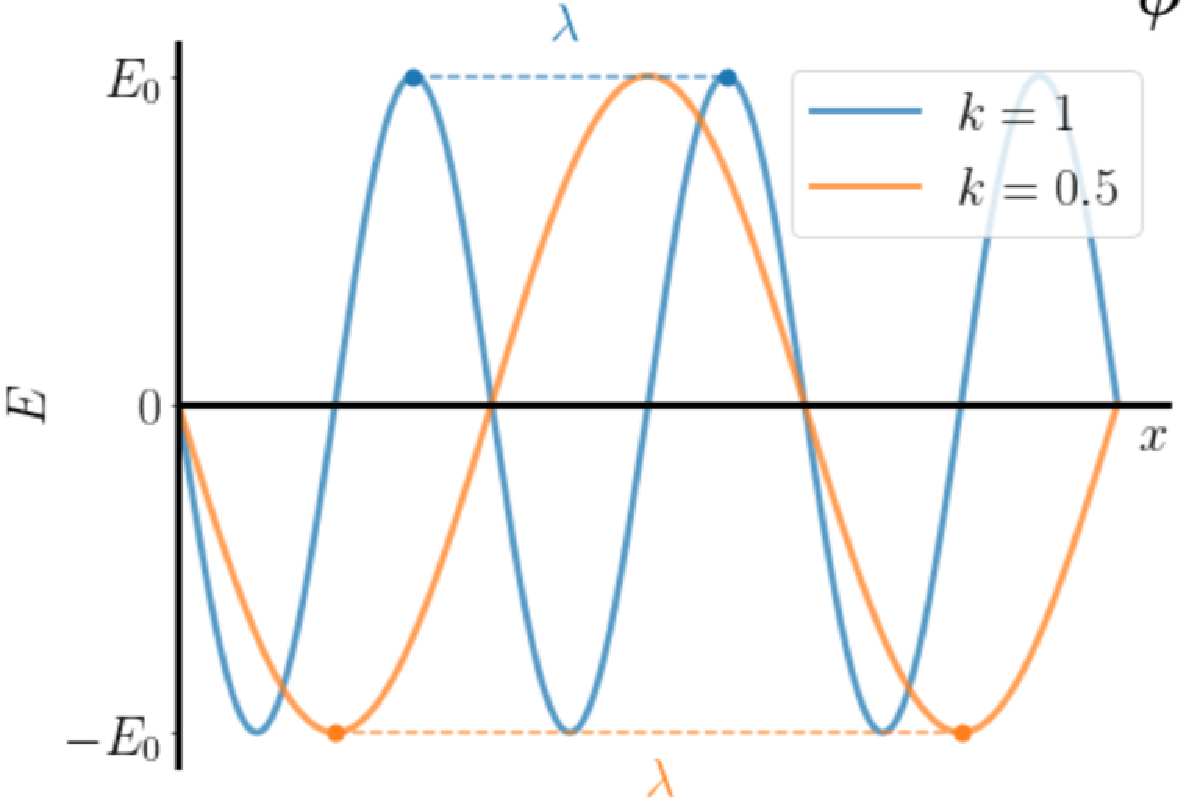
\includegraphics[width=0.8\textwidth]{lesson6/k.pdf}
    \label{fig: 1}
    \begin{center}
        \caption{Wave with $k=1, k=0.5$}
    \end{center}
\end{figure}

then we will move to interference of single photons
and we will conclude with interference of qubits
so let's begin step one constructive and destructive interference
let's consider that we have a single frequency wave propagating in time
how do we write down a mathematical expression that describes the
propagation of such a wave well we do it as follows we denote the wave
with e and it's some constant e naught times the sine of the following argument
where e naught designates the amplitude of

00:01
oscillations that means how far the how much the wave is disturbing
omega is the angular frequency and it determines
how quickly the wave is propagating in time time here is denoted by this small t
k is the wave number it also it's related to
how fast the wave is propagating as well and in three dimensions it also
gives you the direction of propagation however here we're only considering
propagation in one dimension therefore it's just a number
and phi is called the initial phase so omega the angular frequency is
related to the period of oscillations as follows omega is equal to 2 pi over t
whereas k the wave number is related to the wavelength of the oscillations
% phi = 0, phi = pi/2
\begin{figure}[H]
   \centering
    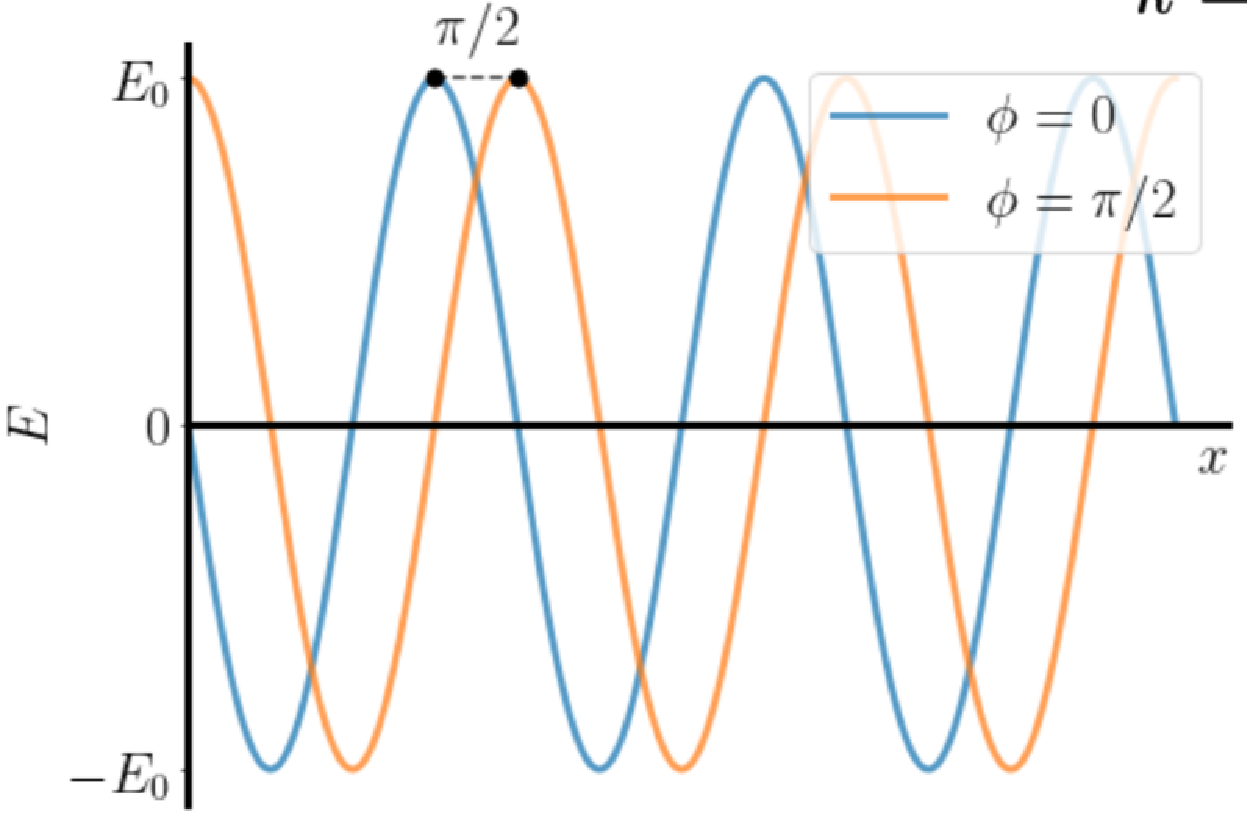
\includegraphics[width=0.8\textwidth]{lesson6/phi.pdf}
    \label{fig: 1}
    \begin{center}
        \caption{$\phi = 0, \phi = \pi / 2$}
    \end{center}
\end{figure}

$\phi = 0$ and $\phi = \frac{\pi}{2}$

00:02
and k is equal to 2 pi over lambda so let's have a look at some examples
for example if we freeze the wave in time so we set
time equals to zero and for convenience we also set phi
equals to zero and we only vary k the blue wave here is for k
equals to one whereas the orange one is for k equals to 0.5
and these two dots the distance between them
represents the wavelength of the wave and as we said the wave number k
is related to the wavelength the larger the wave number is the shorter the
wavelength so we see for k equals to one the wavelength is shorter
than for the other wave where k equals to 0.5 represent it over here
now let's consider what happens when we fix the wave number

% gif two waves [insert pic]
\begin{figure}[H]
   \centering
    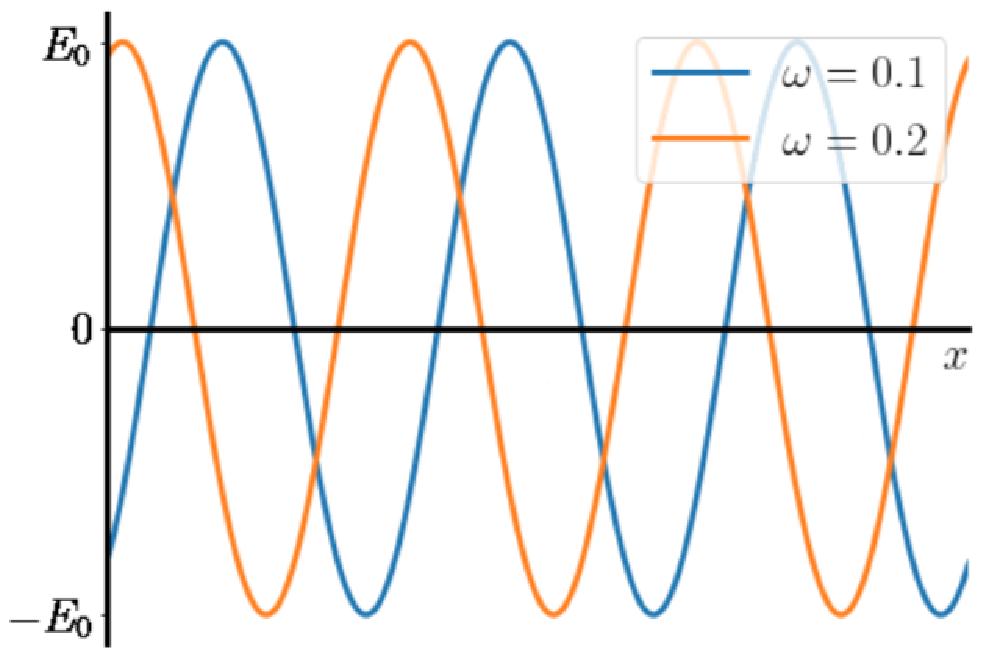
\includegraphics[width=0.8\textwidth]{lesson6/w.pdf}
    \label{fig: 1}
    \begin{center}
        \caption{Wave with $\omega = 0.1, \omega = 0.2$}
    \end{center}
\end{figure}

\begin{equation}
\begin{array}{ll}
E_{1}=E_{01} \sin \left(\omega t+\alpha_{1}\right), & \alpha_{1}=-\left(k x+\phi_{1}\right) \\
E_{2}=E_{02} \sin \left(\omega t+\alpha_{2}\right), & \alpha_{2}=-\left(k x+\phi_{2}\right)
\end{array}
\end{equation}

\begin{equation}
E = E_0 sin(\omega t - \alpha)
\end{equation}

\begin{equation}
\begin{aligned}
E &=E_{01}\left(\sin \omega t \cos \alpha_{1}+\cos \omega t \sin \alpha_{1}\right) \\
&+E_{02}\left(\sin \omega t \cos \alpha_{2}+\cos \omega t \sin \alpha_{2}\right)
\end{aligned}
\end{equation}

\begin{equation}
\begin{aligned}
E &=\left(E_{01} \cos \alpha_{1}+E_{02} \cos \alpha_{2}\right) \sin \omega t \\
&+\left(E_{01} \sin \alpha_{1}+E_{02} \sin \alpha_{2}\right) \cos \omega t
\end{aligned}
\end{equation}

\begin{equation}
\begin{aligned}
&E_{0} \cos \alpha=E_{01} \cos \alpha_{1}+E_{02} \cos \alpha_{2} \\
&E_{0} \sin \alpha=E_{01} \sin \alpha_{1}+E_{02} \sin \alpha_{2}
\end{aligned}
\end{equation}

\begin{equation}
\begin{aligned}
&E_{0}^{2}=E_{01}^{2}+E_{02}^{2}+2 E_{01} E_{02} \cos \left(\alpha_{2}-\alpha_{1}\right) \\
&\tan \alpha=\frac{E_{01} \sin \alpha_{1}+E_{02} \sin \alpha_{2}}{E_{01} \cos \alpha_{1}+E_{02} \cos \alpha_{2}}
\end{aligned}
\end{equation}

\begin{equation}
E = E_0 sin(\omega t + \alpha)
\end{equation}
\begin{equation}
E_{0}^{2}=E_{01}^{2}+E_{02}^{2}+2 E_{01} E_{02} \cos \left(\alpha_{2}-\alpha_{1}\right)
\end{equation}

\begin{equation}
    \delta = 0, \pm2\pi, \pm4\pi, \pm6\pi, \pm8\pi, \pm10\pi
\end{equation}

\begin{equation}
    \delta = \pm1\pi, \pm3\pi, \pm5\pi
\end{equation}

\begin{equation}
\begin{aligned}
&E_{1}=\sin (0.1 t-x) \\
&E_{2}=\sin (0.1 t-0.8 x) \\
&E=E_{1}+E_{2}
\end{aligned}
\end{equation}

% superposition two waves
\begin{figure}[H]
   \centering
    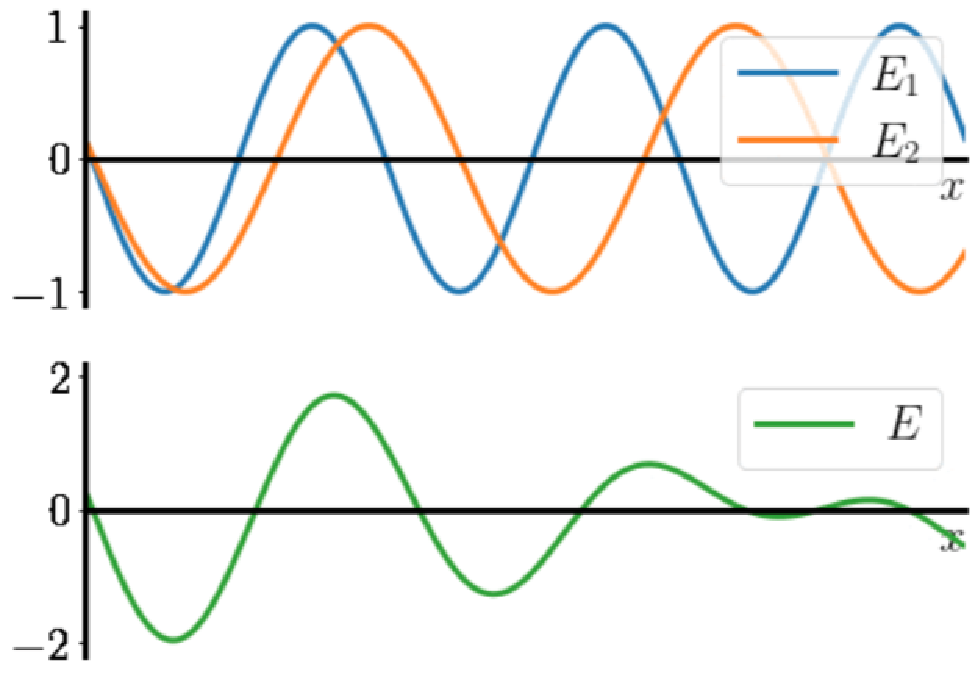
\includegraphics[width=0.8\textwidth]{lesson6/wave_superposition.pdf}
    \label{fig: 1}
    \begin{center}
        \caption{Waves in superposition}
    \end{center}
\end{figure}

00:03
but we vary the initial phase the only thing that happens
is that we shift the wave along the x-axis so really what we are doing we
are just translating the wave a little bit by this angle
by this initial phase phi so in this case we have shifted
the two waves by uh initial phase of pi over two but this doesn't really affect
how fast the wave is propagating or it doesn't affect its um um its wavelength
so finally let's add time independ time dependence into the picture
we set k equals to one and we also set the initial phase
phi to be zero and now the wave is actually propagating in time
here we have two waves again for the first wave represented by the blue
we have omega equals to 0.1 whereas for the second wave

00:04
we've got 0.2 remember we said that omega determines how fast
the wave is propagating in time and we can clearly see that the orange wave
is faster than the blue wave so now let's consider two waves that are
actually interacting together and creating a new third wave how do we
how do we describe this new disturbance so let's say that we've got two waves e1
and e2 each with different amplitude same frequency and
we grouped the spatial depend spatial variation into these factors
alpha alpha 1 and alpha 2. and to get this new wave that e1 and e2 produce
is actually relatively simple you just add them together and this is known as
the principle of superposition and the idea is

00:05
that we are looking for a description of the new
resultant wave also in this form where now we have to
find out what is this new amplitude e naught in terms of uh in terms of the
composite waves and also we want to find out this new factor of alpha
so let's see how we can do that what we do is
we just add the two waves together and we begin by expanding
these signs so the first wave can be written as this
we have the initial amplitude of the first wave e
0 1 and then we've got sine omega t times cos alpha 1 plus cos omega t
times sine alpha 1 and similarly for the second wave so we add them
together and now what we do is we group the time dependent terms so we see
that these two terms they both vary in time as sine omega t

00:06
whereas these two terms vary as cos omega t so let's group them together
and we get the following expression we've got some spatial
variation here times sine omega t and another spatial variation here times cos
omega t and what we can do now is we can define e naught cos alpha
s this whole first expression and e naught sine alpha as the second expression
and now with a little bit of algebra what we arrive at is
are the following expressions so if we square this first expression and add it
to the square of the second expression cos squared alpha plus sine squared
alpha is equal to one that's a very important trigonometric
identity so on this side we get e naught squared and then we just have
the squares which we have expanded over here
and simplified with some trigonometric identities

00:07
also if we take this orange expression the second expression over here
and we divide by this blue expression over here
we can get an expression for tangent of alpha given as this following
ratio and this is our new wave so we started with two waves with same
frequencies which means that the the resultant disturbance also
travels at the same frequency which makes sense but this new wave has different
amplitude and also different phase so let's look at some examples but
before that actually let's look at the let's look at the
amplitude of the superposition so we've got the amplitude squared is
equal to the sum of the squares of the component amplitudes which makes sense
but then there is this extra term and this extra term is very important
it's called the interference term you can see that it actually
oscillates as a result of the difference

00:08
between alpha two and alpha one and this this difference is called the phase
difference so the entire expression for e naught
squared is maximized when delta is either zero
or multiples of two pi and we call this constructive interference because it's
adding to the new resultant amplitude on the other hand if the phase difference
is an integer multiple of pi as plus or minus pi or plus or minus 3 pi
then what we get is destructive interference because
this interference term over here is minimized
so let's look at some examples we've got two waves
we set their amplitudes to be equal for convenience both are one
their omegas are the same 0.1 and the only thing that is different
between them are the wave numbers k for the first wave k equals

00:09
1 for the second wave k equals 0.8 so we add the two together and what we get
is the following here with this blue and orange waves we see the waves traveling
independently whereas the green wave is the superposition of these two waves
and you can see the interference at play at the beginning
over here where x is small in this region
the waves travel in such a way that the crest seems to be on top of the
crest of the other wave therefore we get constructive uh interference the waves
are reinforcing each other they're adding together producing something larger
whereas as the wave propagates into this uh
region of larger x they are propagating at different
speed so what happens they go out of phase so the crest of one wave
is meeting the trough of the other wave so they are destructively interfering
and they're cancelling each other out and you can see that in this
green wave where the amplitude becomes very very low

00:10
nearly zero and that's how interference works

\section{Phase and group velocities}

\begin{equation}
E=E_{0} \sin (\omega t-k x-\phi)
\end{equation}


$\theta=\omega t-k x-\phi$

\begin{equation}
E=\sin (0.1 t-x)
\end{equation}

% graph, black dot
\begin{figure}[H]
   \centering
    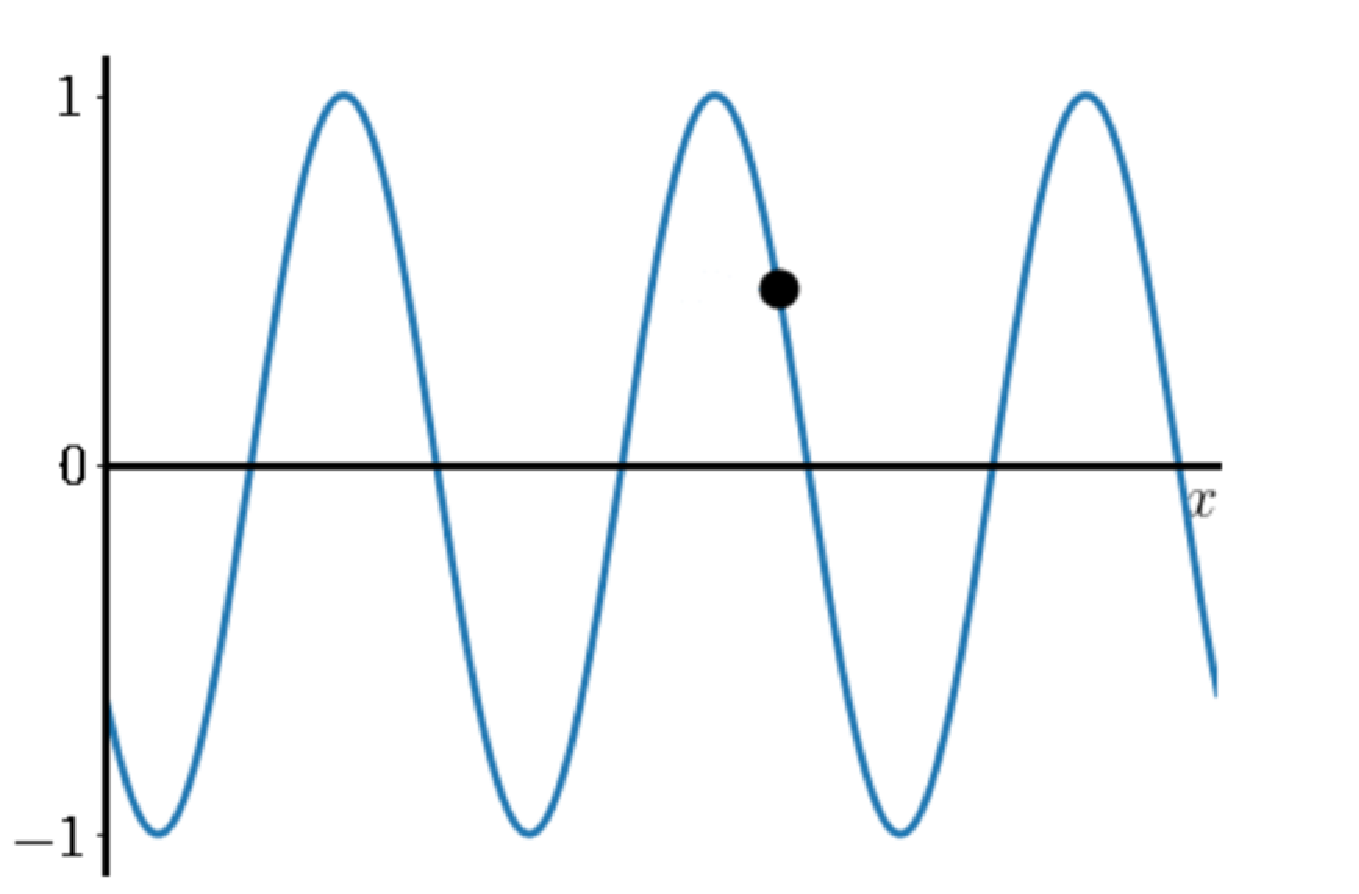
\includegraphics[width=0.8\textwidth]{lesson6/black_dot.pdf}
    \label{fig: 1}
    \begin{center}
        \caption{Phase velocity of a single wave.}
    \end{center}
\end{figure}

\begin{equation}
\begin{aligned}
&E_{1}=E_{0} \sin \left(\omega_{1} t-k_{1} x\right) \\
&E_{2}=E_{0} \sin \left(\omega_{2} t-k_{2} x\right)
\end{aligned}
\end{equation}

\begin{equation}
\begin{aligned}
E &=E_{1}+E_{2} \\
&=E_{0}\left[\sin \left(\omega_{1} t-k_{1} x\right)+\sin \left(\omega_{2} t-k_{2} x\right)\right] \\
&=2 E_{0} \sin \left[\frac{\omega_{1}+\omega_{2}}{2} t-\frac{k_{1}+k_{2}}{2} x\right] \\
& \times \cos \left[\frac{\omega_{1}-\omega_{2}}{2} t-\frac{k_{1}-k_{2}}{2} x\right]
\end{aligned}
\end{equation}

\begin{equation}
E=2 E_{0} \sin \left[\frac{\omega_{1}+\omega_{2}}{2} t-\frac{k_{1}+k_{2}}{2} x\right] \times \cos \left[\frac{\omega_{1}-\omega_{2}}{2} t-\frac{k_{1}-k_{2}}{2} x\right]
\end{equation}

\begin{equation}
v_p = \frac{\omega_{1}+\omega_{2}}{k_{1}+k_{2}}
\end{equation}

\begin{equation}
v_g = \frac{\omega_{1}-\omega_{2}}{k_{1}-k_{2}}
\end{equation}

\begin{equation}
\begin{aligned}
&E_{1}=\sin (0.1 t-2.0 x) \\
&E_{2}=\sin (0.2 t-2.1 x)
\end{aligned}
\end{equation}

% t = 0 graph
\begin{figure}[H]
   \centering
    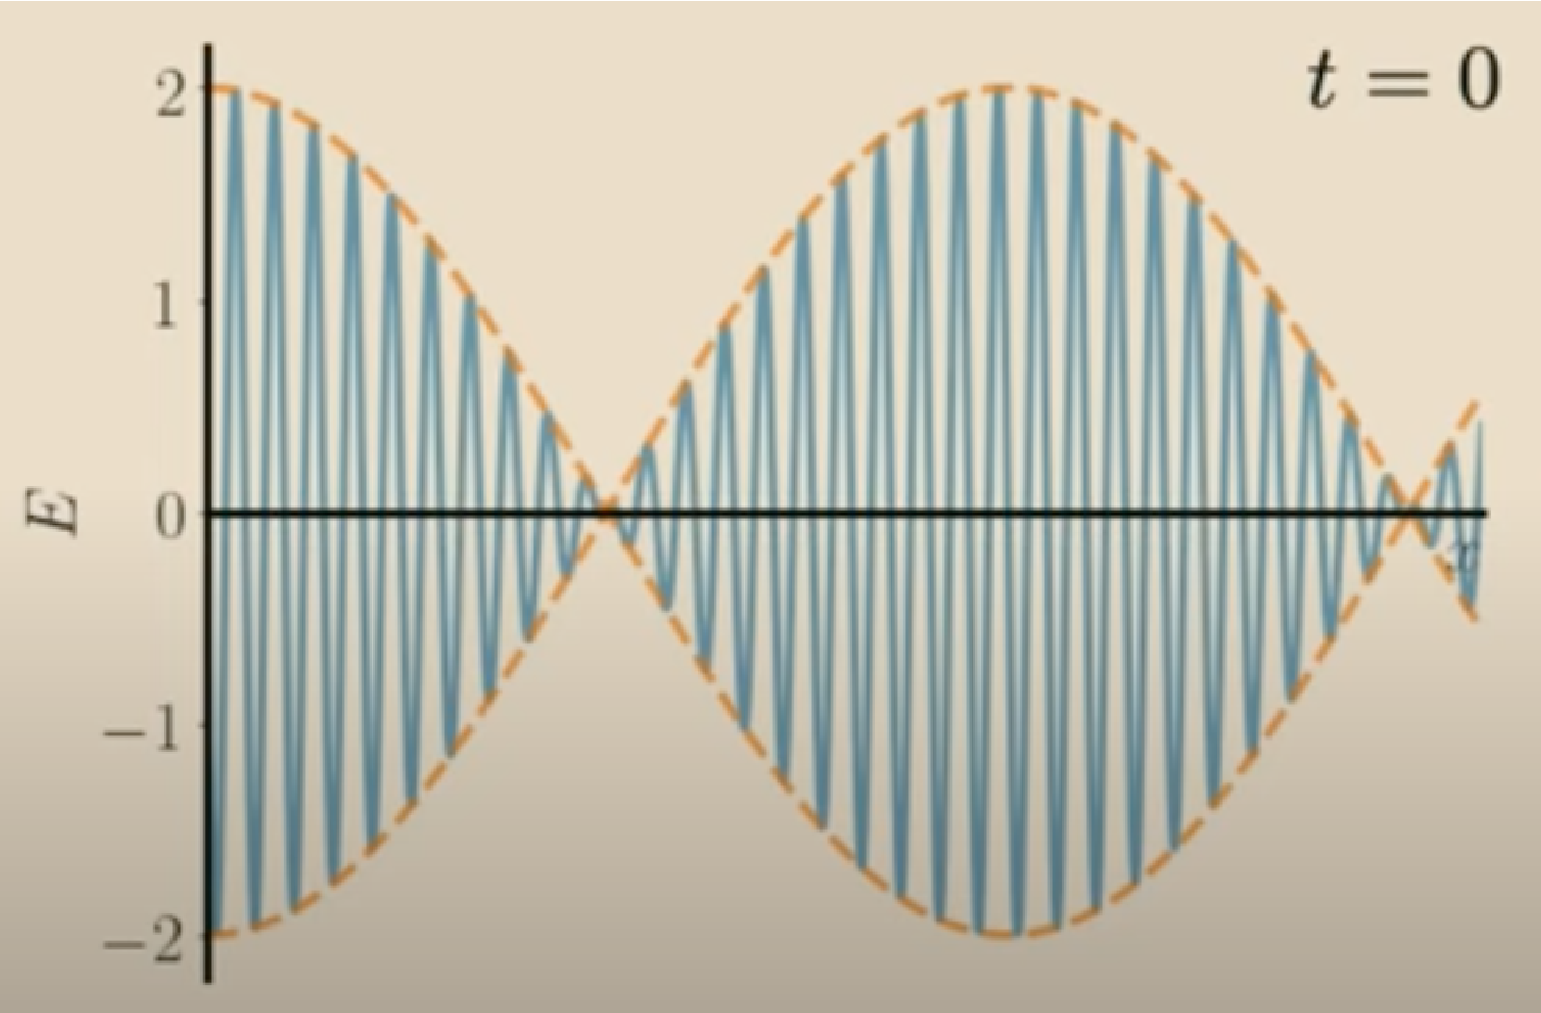
\includegraphics[width=0.8\textwidth]{lesson6/t=0.pdf}
    \label{fig: 1}
    \begin{center}
        \caption{}
    \end{center}
\end{figure}

\begin{equation}
\begin{gathered}
v_{p}=\frac{\omega_{1}+\omega_{2}}{k_{1}+k_{2}}=\frac{0.3}{4.1} \approx 0.07 \\
%v_{g}=\frac{\omega_{1}-\omega_{2}}{k_{1}-k_{2}}=1 & 
v_{g}=\frac{\omega_{1}-\omega_{2}}{k_{1}-k_{2}}=1 
\begin{array}{l}
\end{array} \\
v_{g}>v_{p} \quad v_{g} \approx 14 v_{p}
\end{gathered}
\end{equation}

% red square, black dot
\begin{figure}[H]
   \centering
    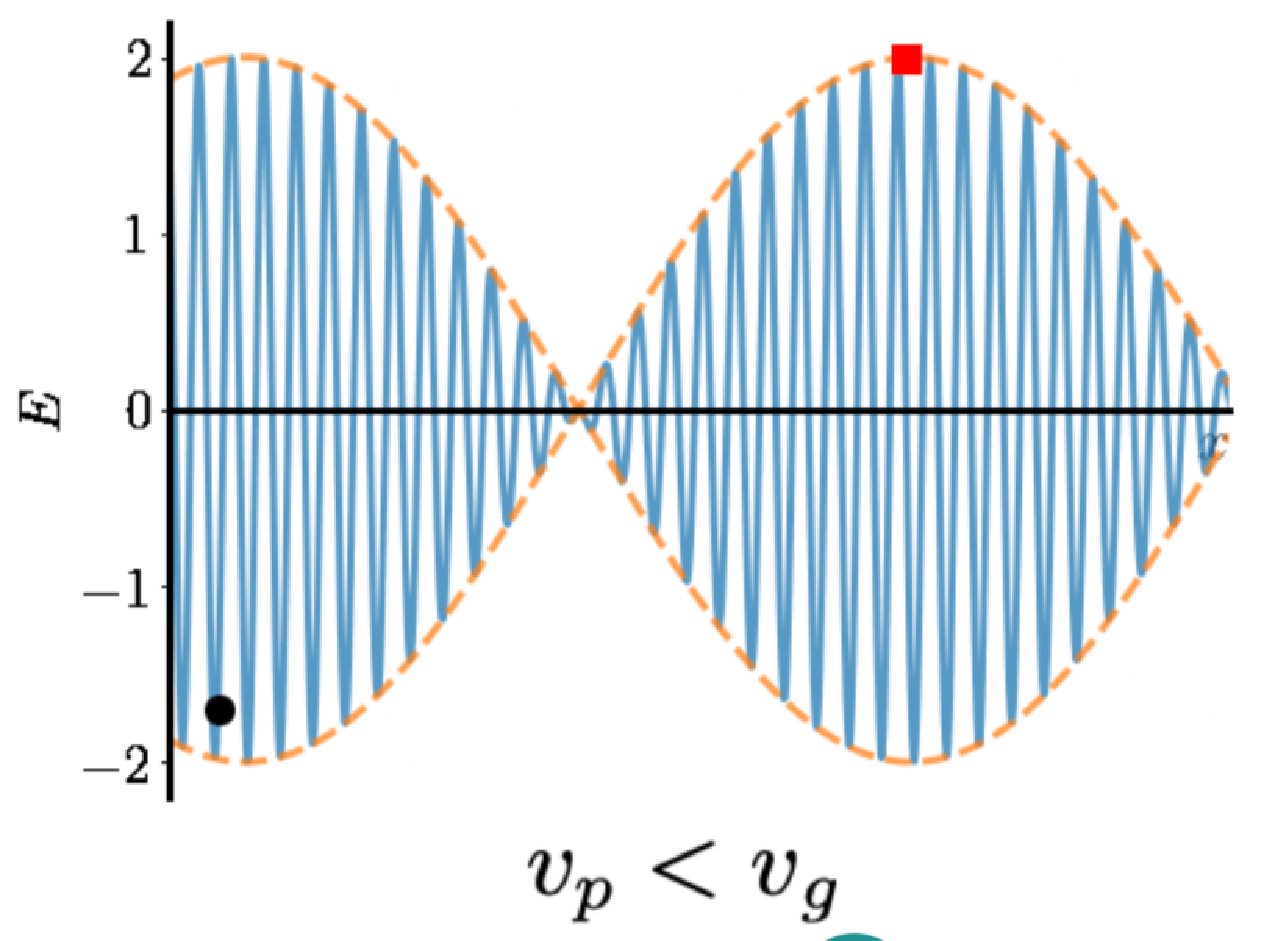
\includegraphics[width=0.8\textwidth]{lesson6/vp_less_vg.pdf}
    \label{fig: 1}
    \begin{center}
        \caption{A superposition with $v_p < v_g$.}
    \end{center}
\end{figure}

\begin{equation}
\begin{aligned}
&E_{1}=\sin (0.1 t-0.1 x) \\
&E_{2}=\sin (0.2 t-0.2 x)
\end{aligned}
\end{equation}

% vp = vg
\begin{figure}[H]
   \centering
    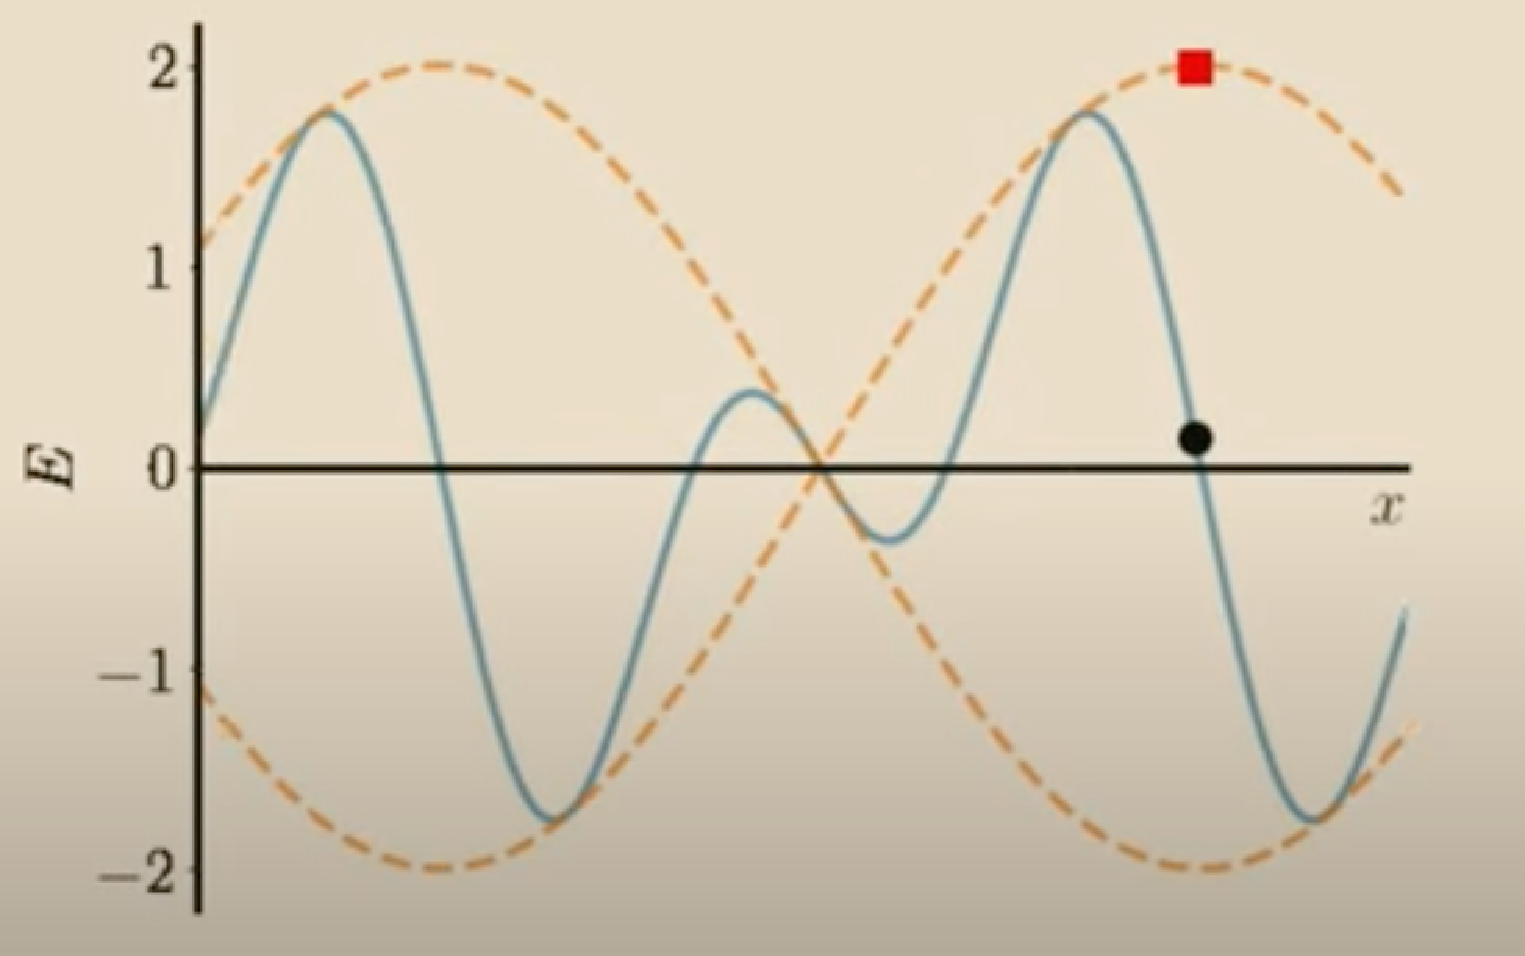
\includegraphics[width=0.8\textwidth]{lesson6/vp_equal_vg.pdf}
    \label{fig: 1}
    \begin{center}
        \caption{A superposition with $v_p = v_g$}
    \end{center}
\end{figure}

\begin{equation}
\begin{aligned}
&E_{1}=\sin (0.1 t-2.0 x) \\
&E_{2}=\sin (0.2 t-1.5 x)
\end{aligned}
\end{equation}
% vg < vp
\begin{figure}[H]
   \centering
    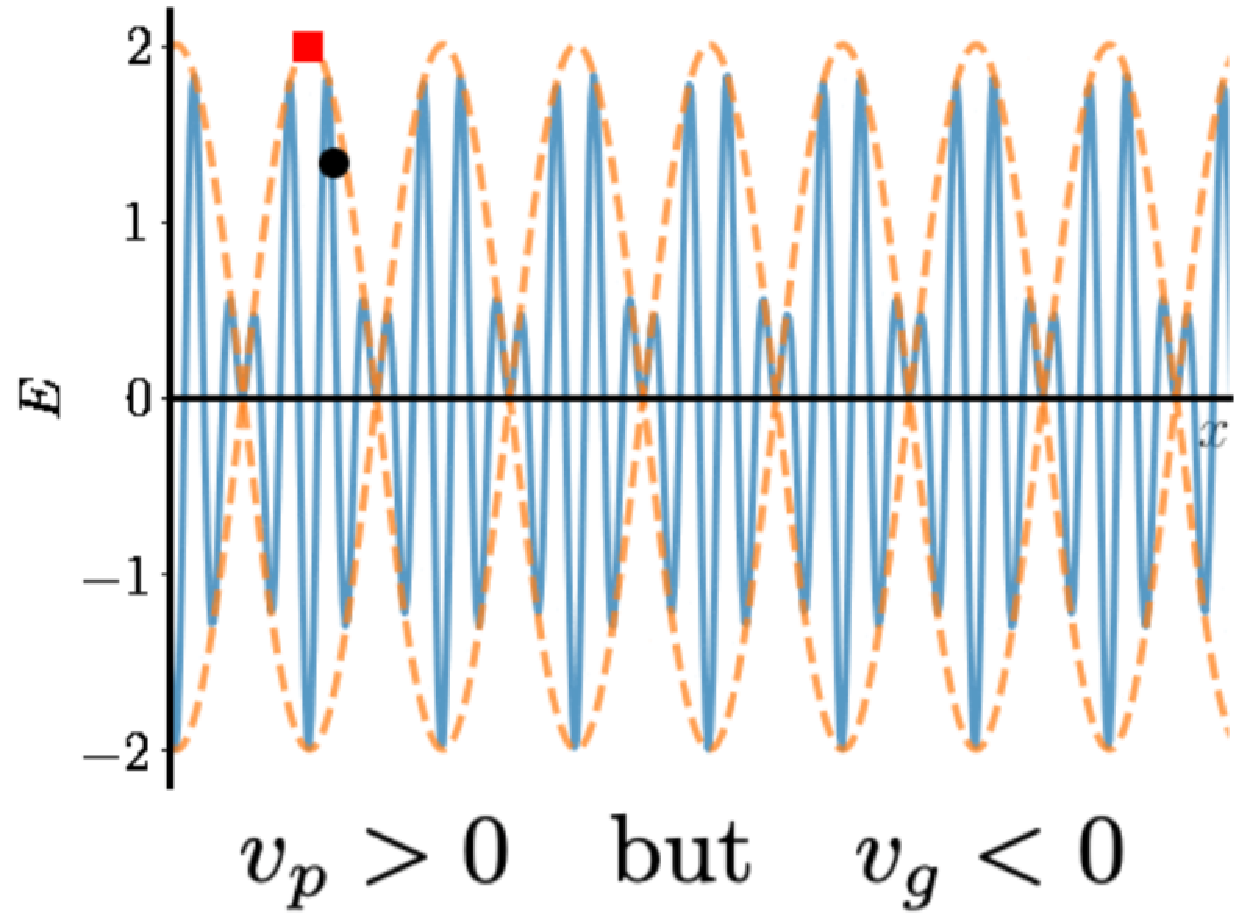
\includegraphics[width=0.8\textwidth]{lesson6/vp_greater_vg.pdf}
    \label{fig: 1}
    \begin{center}
        \caption{A superposition with $v_p > v_g$.}
    \end{center}
\end{figure}

\begin{equation}
\begin{aligned}
E &=\sum_{k=2}^{3} \sin (-k x), \quad k \text { increasing in steps of } 0.1 \\
&=\sin (-2.0 x)+\sin (-2.1 x)+\ldots+\sin (-3.0 x)
\end{aligned}
\end{equation}

% pulse
\begin{figure}[H]
   \centering
    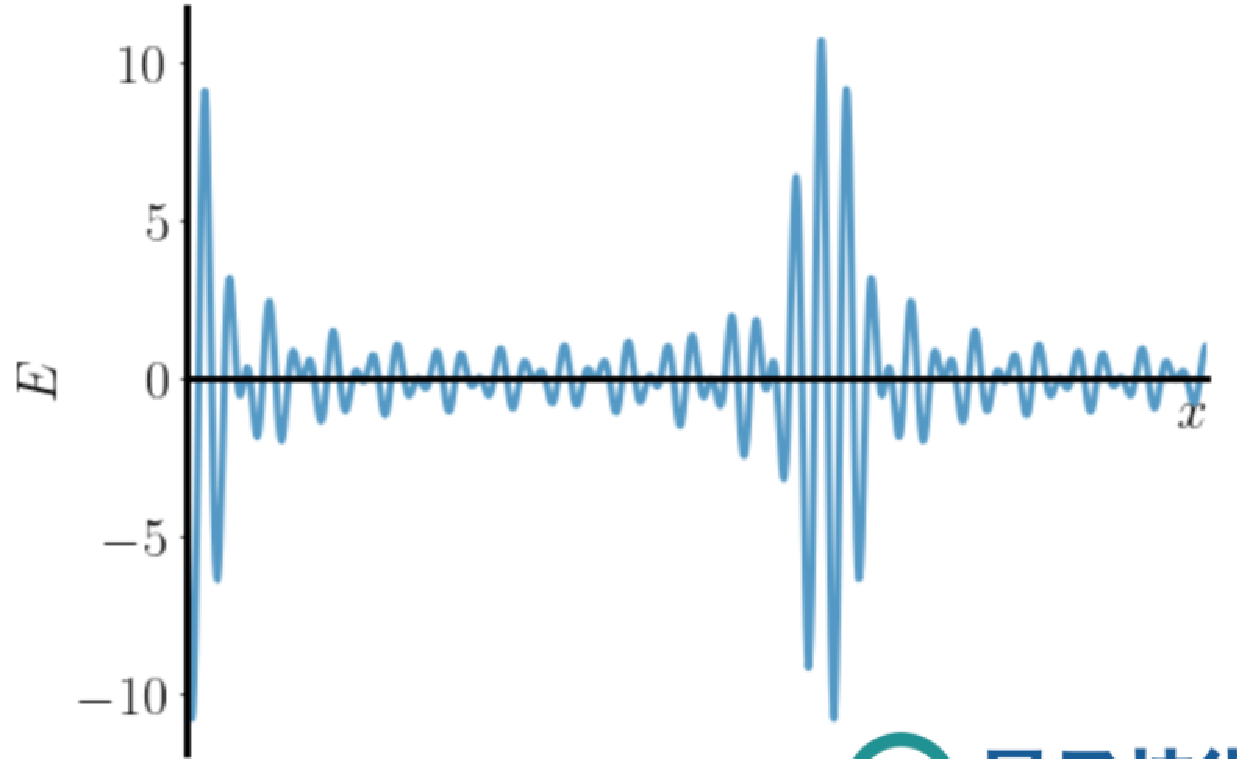
\includegraphics[width=0.8\textwidth]{lesson6/pulse.pdf}
    \label{fig: 1}
    \begin{center}
        \caption{}
    \end{center}
\end{figure}


00:00
step 2 base and group velocities in this step we will get back to
interference and see what effect it has on the speed with which waves propagate
so first let's consider a single wave of a single frequency
propagating through space and ask the question
at what speed does this wave travel we saw in the previous step that we can
write down such a wave in this form we've got the amplitude times sine of
its phase and maybe you remember from previous studies
that the wave velocity is given as the ratio of the
wavelength lambda and its period capital t so we saw in the previous step that
lambda is related to the wave number k as follows lambda is equal to 2 pi over

00:01
k and similarly the period of oscillation capital t is related to omega
the angular frequency as 2 pi over omega so substituting for lambda and
substituting for t we can obtain the expression for wave velocity
in terms of omega and k as v the wave velocity is omega over k
so now we know how a single wave propagates let's consider when we have
two waves that superpose together before we do that let's look at an
example so we have a wave propagating at angular frequency 0.1
and the wave number is 1. and then as you can see i marked one black point here
this is a point of constant phase and it's propagating
through through space like that so now what happens when we superpose two waves

00:02
how at what velocity and what speed does the resultant superposition travel
well let's take two waves and this time we allow their angular frequencies to be
different their wave numbers to be different but
for simplicity we consider these two waves to have same amplitude e naught
when we add them together we arrive at the
following expression here both of them have some amplitude so
we can just take out e naught out and write down the two waves in this form
and what we do next is we apply a trigonometric identity that
allows us to write this superposition e as a product
of two wave signals one is a sine signal and the other one is a cos signal
for the sine the angular frequency is the following omega 1 plus omega 2 over 2
and the new wave number is k1 plus k2 over 2 and for the cos signal we take the

00:03
difference of the angular frequencies omega 1 and omega 2 and the wave numbers
k1 and k2 so let's have a look at the shape of this superposition
we said that we've got these two terms that determine
our superposition if we only look at the sign
we see that it's oscillating at a much faster
uh frequency because here we are adding adding the uh angular velocities omega
1 and omega 2 and we are adding the wave numbers
k1 and k2 whereas the other term the cosine term we call that the slow
oscillating term because the angular the new angular frequency is dependent
on the difference between omega 1 and omega 2 and the difference between k1
and k2 so we define the phase velocity as the velocity of this

00:04
fast oscillating term so previously we said that for a single wave it's just
omega over k but here we saw that this omega ones and omega twos result in this
new angular frequency for the fast oscillations
and this new wave number for the fast oscillations
so vp the phase velocity is equal to as omega 1 plus omega 2 divided by k1
plus k2 and the group velocity is defined in a similar way but for the
slow oscillations so vg which we denote group velocity
is omega 1 minus omega 2 divided by k1 minus k2 so from this you can
immediately see that even though we have a single wave single superposition
there are these two notions of a phase velocity and group velocity
which are not necessarily the same they can be different
and we will see that later in this step so let's illustrate it within with an

00:05
example we consider two waves e1 and into e2
they have different angular frequencies e1 has angular frequency 0.1
whereas e2 has angular frequency 0.2 and they have different
wave numbers e1 has 2.0 and e2 has 2.1 so let's plot this
initially at time equals to zero and we see as we said
we expect the shape of the superposition to to be composed of two waves
one is this fast oscillating blue line and on top of that we have this
slowly varying envelope again this blue fast oscillating term is
given by the sine sine term from previous slides and this orange
dashed line gives us the envelope which is proportional to the cosine

00:06
now let's get things moving and in time again it propagates through space
so now let's actually compute what the phase and group velocities are
for our example we just substitute into our expressions
for uh phase velocity so omega 1 plus omega 2
we just add them together so 0.1 plus 0.2 is 0.3 k1 plus k2
again we add them together 2.0 plus 2.1 is 4.1 and this is approximately 0.07
for the group velocity we do the same thing and we obtain that the group
velocity is equal to 1. so we can see that the group velocity in
this case is larger than the phase velocity
and in fact it's about 14 times larger so let's get back to our propagating
wave and here you can see what actually happens to the points

00:07
uh on on our wave so this black dot oscillating up and down represents
our phase velocity this black point is moving
through space with the phase velocity so
you can see that it's moving up and down quite a lot but actually it's not
propagating through space very much because it's in this example equal to 0.07
whereas this red square that occasionally you can see at the top
that goes zooming uh um see it's sitting on the envelope over there and it goes
to zooming through space that point represents the group velocity
well you can actually see that it's 14 times faster but
mathematically that's true and as we said in this case that we picked the phase
velocity is smaller than the group velocity
but this is not always the case let's look at this following example
we kept the same angular frequencies for the two waves but
we changed the wave numbers now e1 has k equal to 0.1 and e2 has k equal to 0.2

00:08
let's see what what that looks like as you can see
now the group velocity and the phase velocity are the same
the black point and the red square move at the same velocity
so far we have looked at cases when both velocities
are in the same direction now let's look at a very peculiar case
again we keep the angular frequencies fixed but this time we change k1 to 2.0
and k2 to 1.5 and let's see what happens you see that again the black dot
representing our phase velocity is moving in the positive x direction
as was the case before but on the other hand this red square
is moving backwards because the group velocity in this case
is actually negative so you can see that
you can have a lot of fun with the group and phase velocities there are many

00:09
different scenarios depending on omega 1 and omega 2 and k1 and k2
and so far we have been looking at superposition of only two waves
what happens if we consider superposition of more than two waves
let's consider a particular example where our superposition
is given as a sum of some very simple waves
here we have a frozen time and basically set t equals to zero
so we only have sine of minus kx where this k's vary from 2 to 3 in steps of 0.1
so really what we have is a sum of sine of minus 2x plus a sine of minus 2.1
x and so on until we reach the 11th term of sine minus 3x
and in fact what we get is the following following shape
what we call this shape is a pulse you can see that

00:10
for most of x the superposition is close to zero there's there are some
disturbances there are some oscillations but they're
close to zero and then suddenly constructive interference kicks in and
you have this big pulse over there and pulses are very important because
using pulses we can in encode information so it's
very important in communication theory

\section{Interference with single photons}

% double_slit standard
\begin{figure}[H]
   \centering
    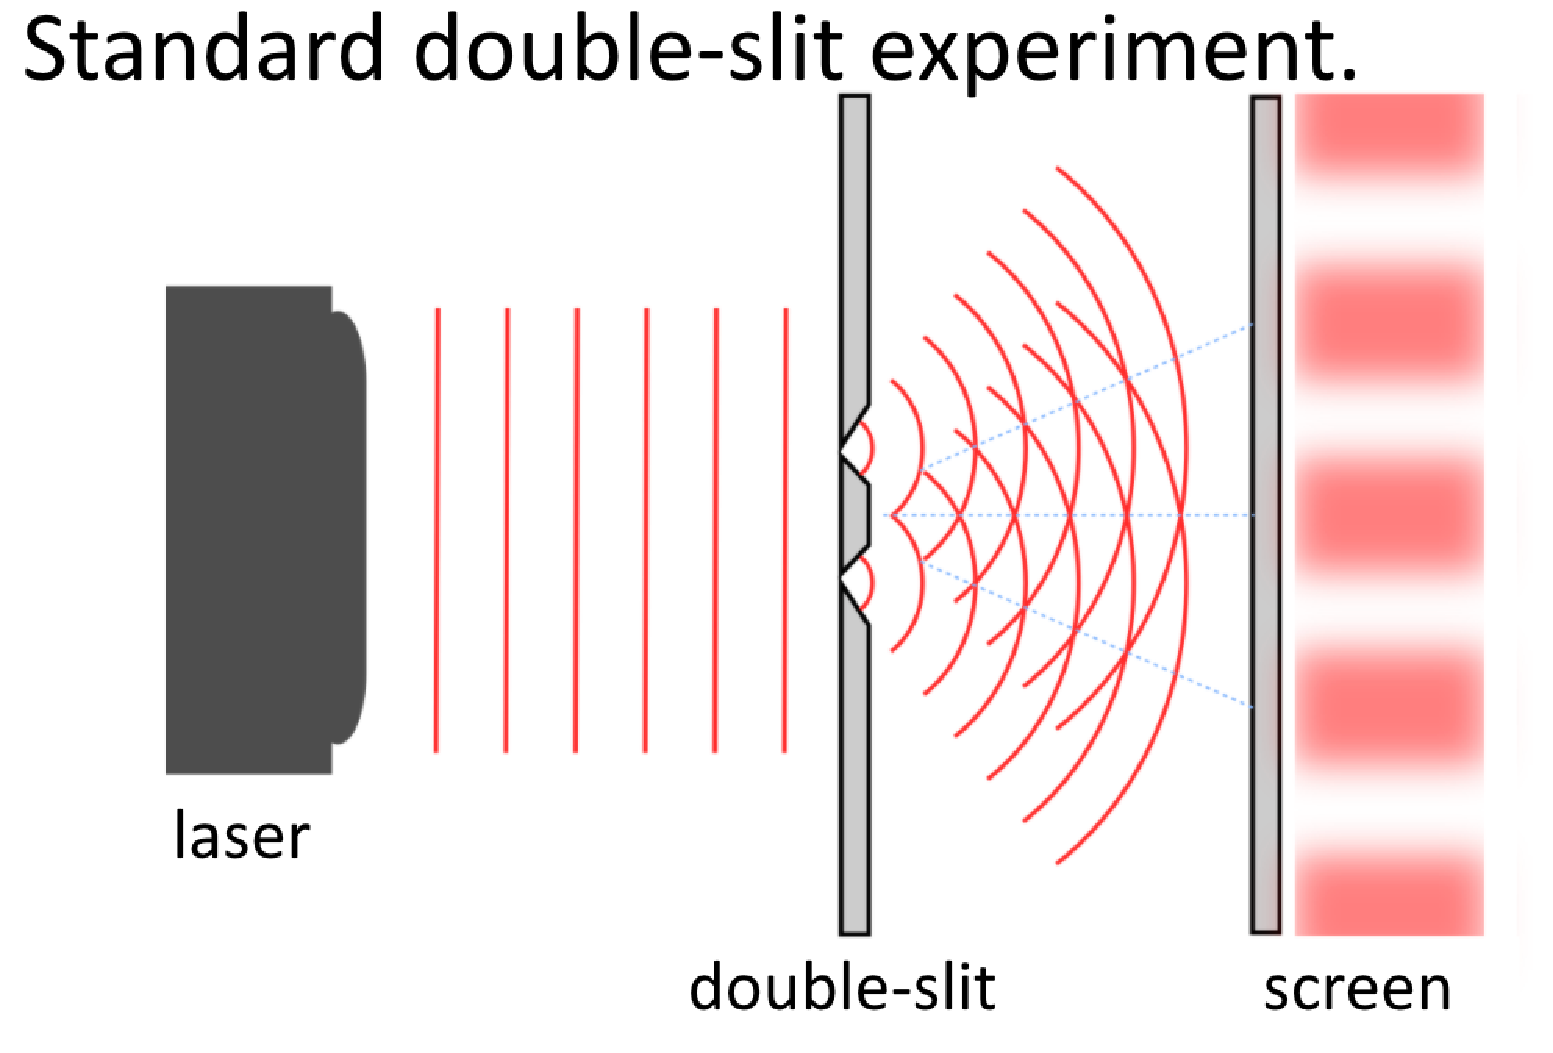
\includegraphics[width=0.8\textwidth]{lesson6/standard_double_slit.pdf}
    \label{fig: 1}
    \begin{center}
        \caption{The canonical two-slit experiment.}
    \end{center}
\end{figure}

% constructive interference
\begin{figure}[H]
   \centering
    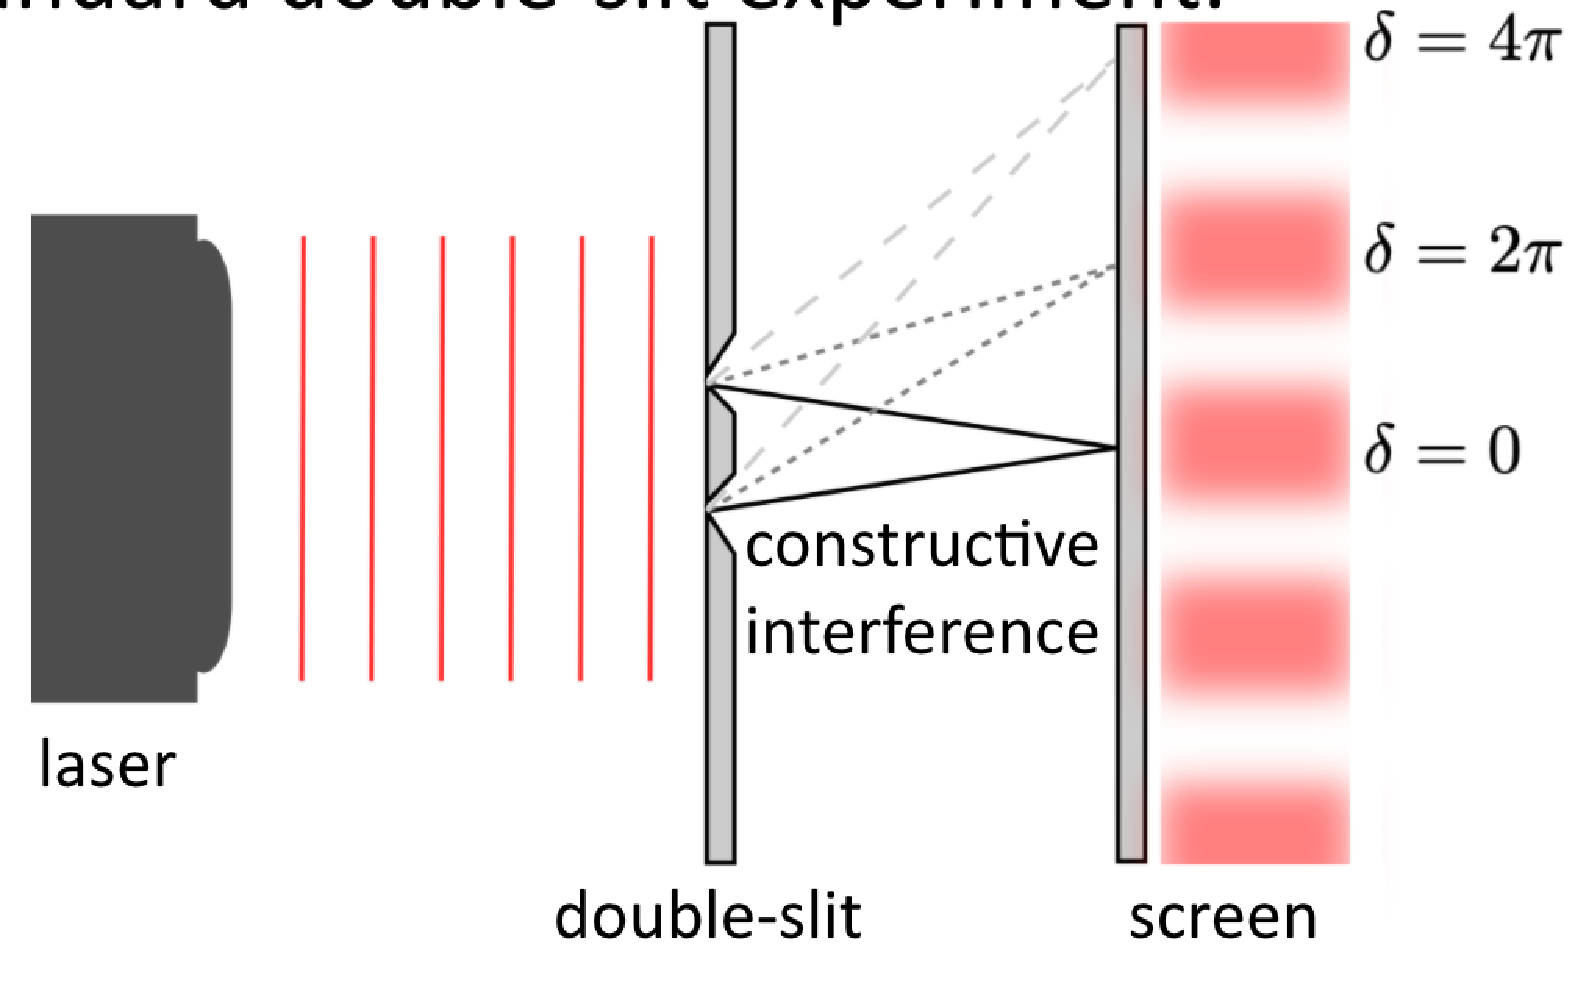
\includegraphics[width=0.8\textwidth]{lesson6/double_slit_constructive.pdf}
    \label{fig: 1}
    \begin{center}
        \caption{Constructive interference.}
    \end{center}
\end{figure}

% destructive inteference
\begin{figure}[H]
   \centering
    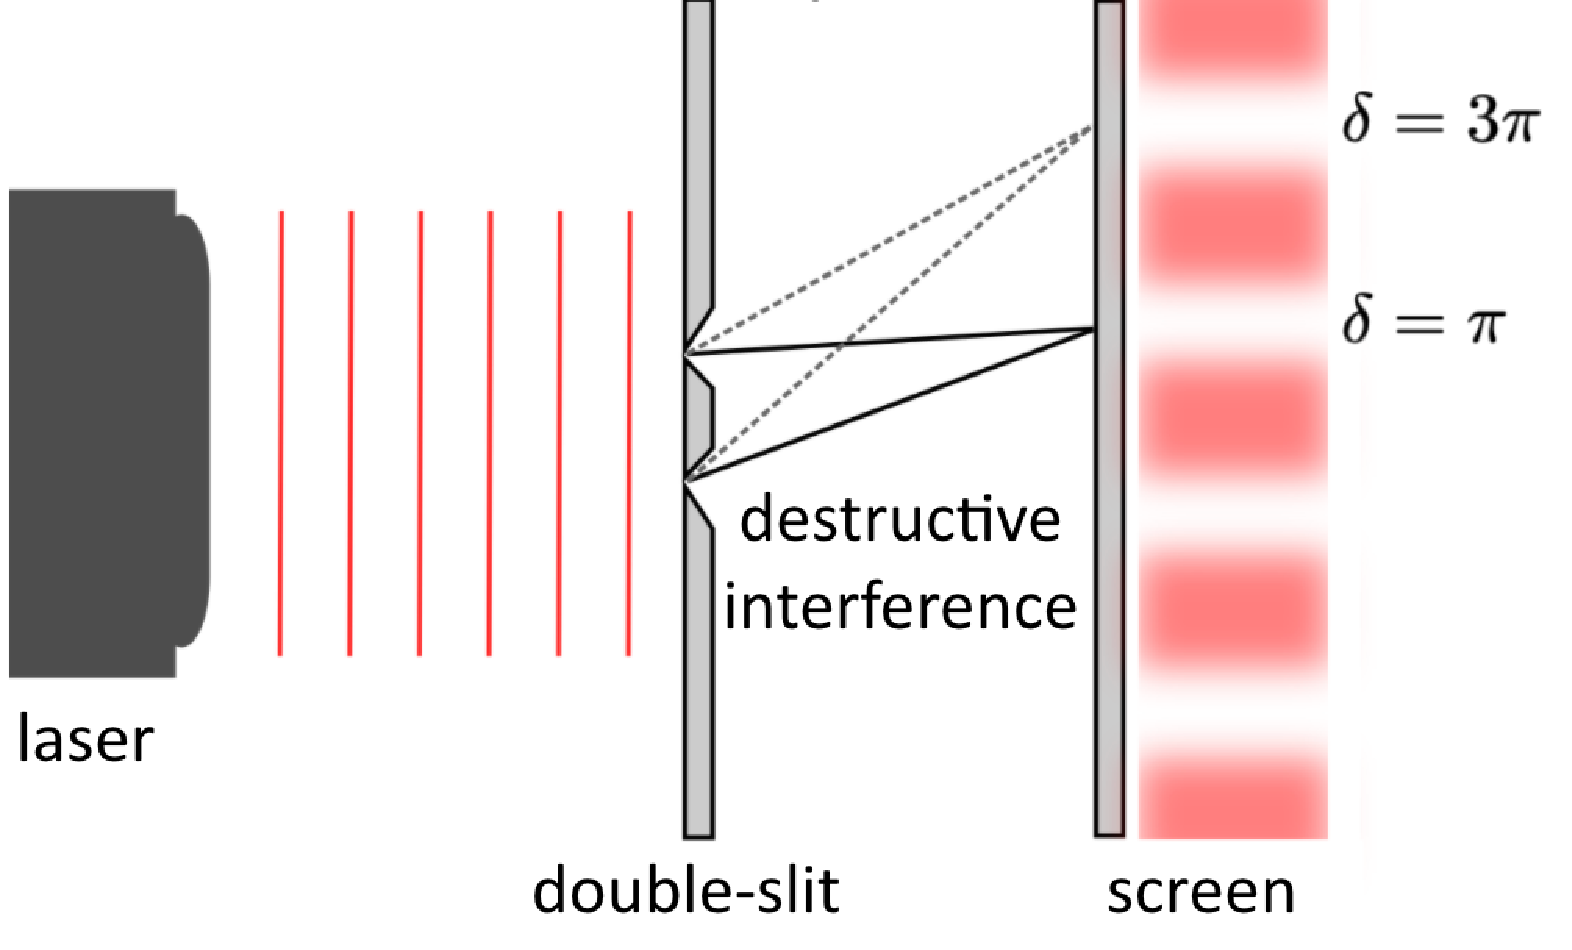
\includegraphics[width=0.8\textwidth]{lesson6/double_slit_destructive.pdf}
    \label{fig: 1}
    \begin{center}
        \caption{Destructive interference.}
    \end{center}
\end{figure}

% attenuated laser
\begin{figure}[H]
   \centering
    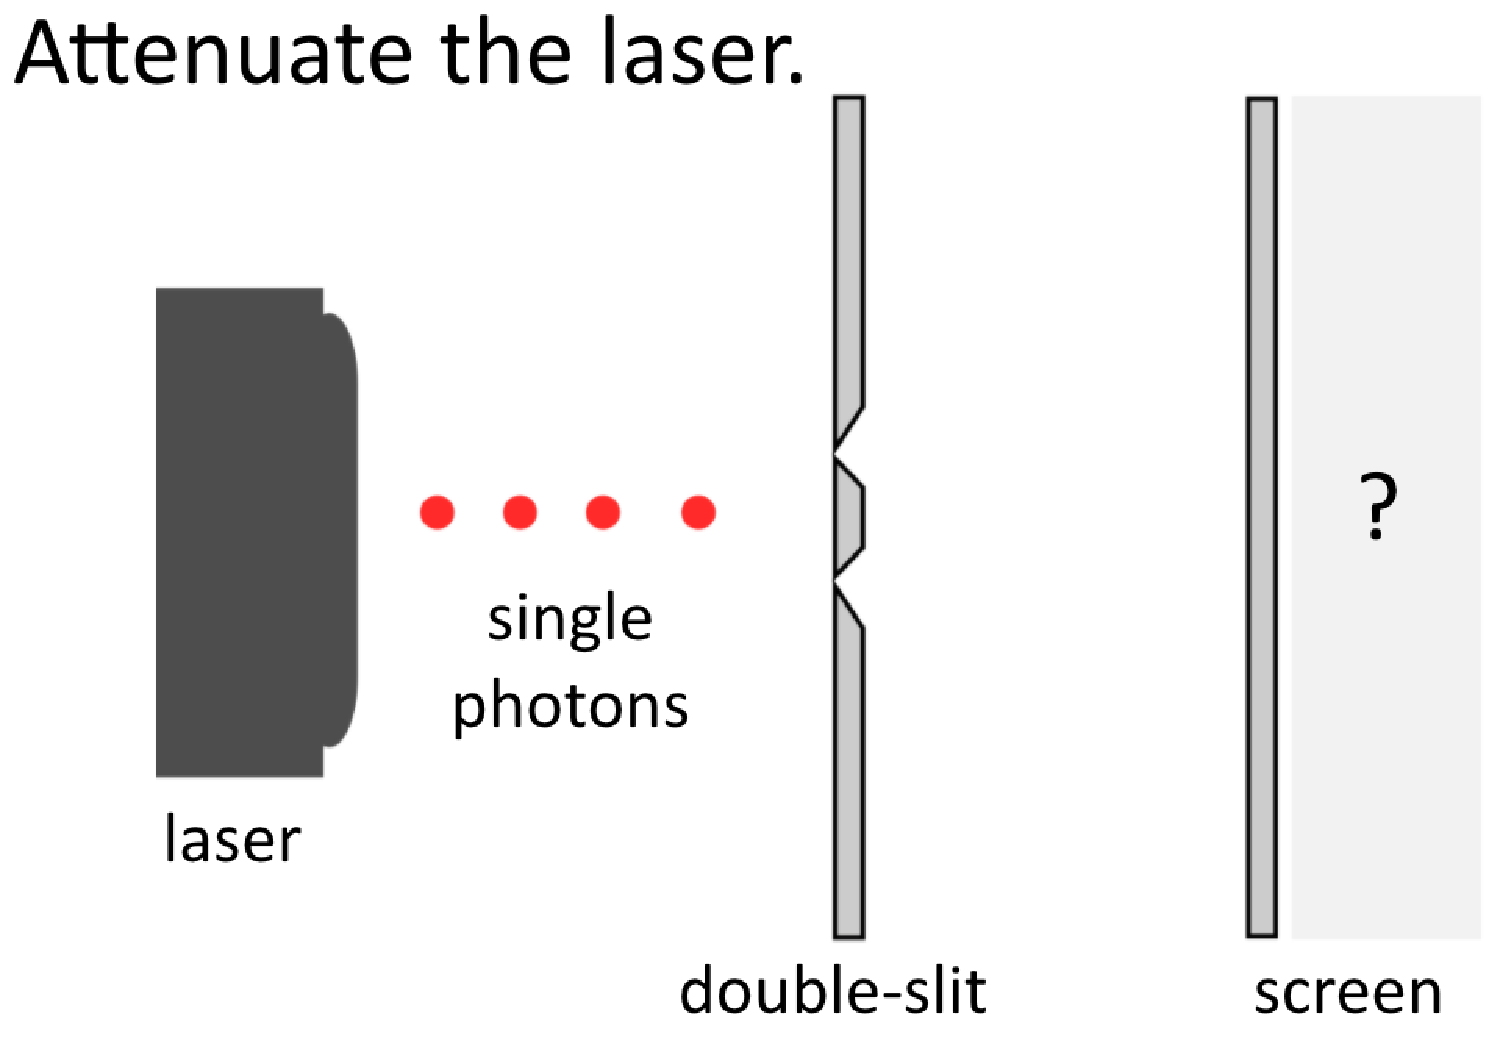
\includegraphics[width=0.8\textwidth]{lesson6/attenuate_laser.pdf}
    \label{fig: 1}
    \begin{center}
        \caption{Attenuated laser light.}
    \end{center}
\end{figure}

% block bottom
\begin{figure}[H]
   \centering
    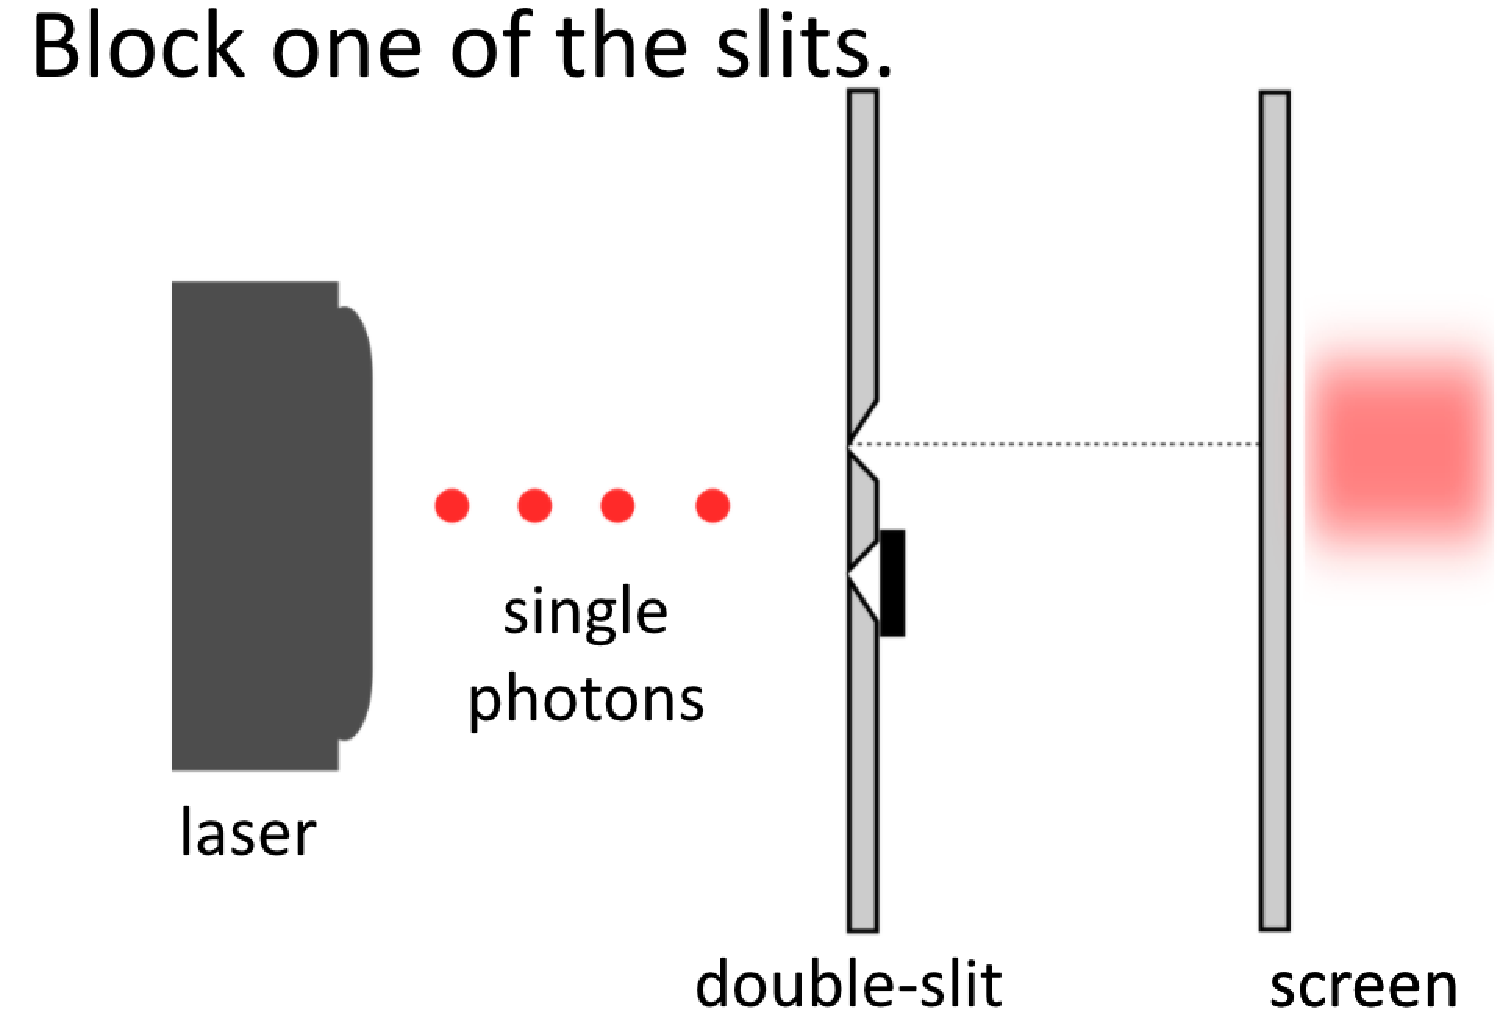
\includegraphics[width=0.8\textwidth]{lesson6/block_bottom.pdf}
    \label{fig: 1}
    \begin{center}
        \caption{Bottom of the block?}
    \end{center}
\end{figure}

% block top
\begin{figure}[H]
   \centering
    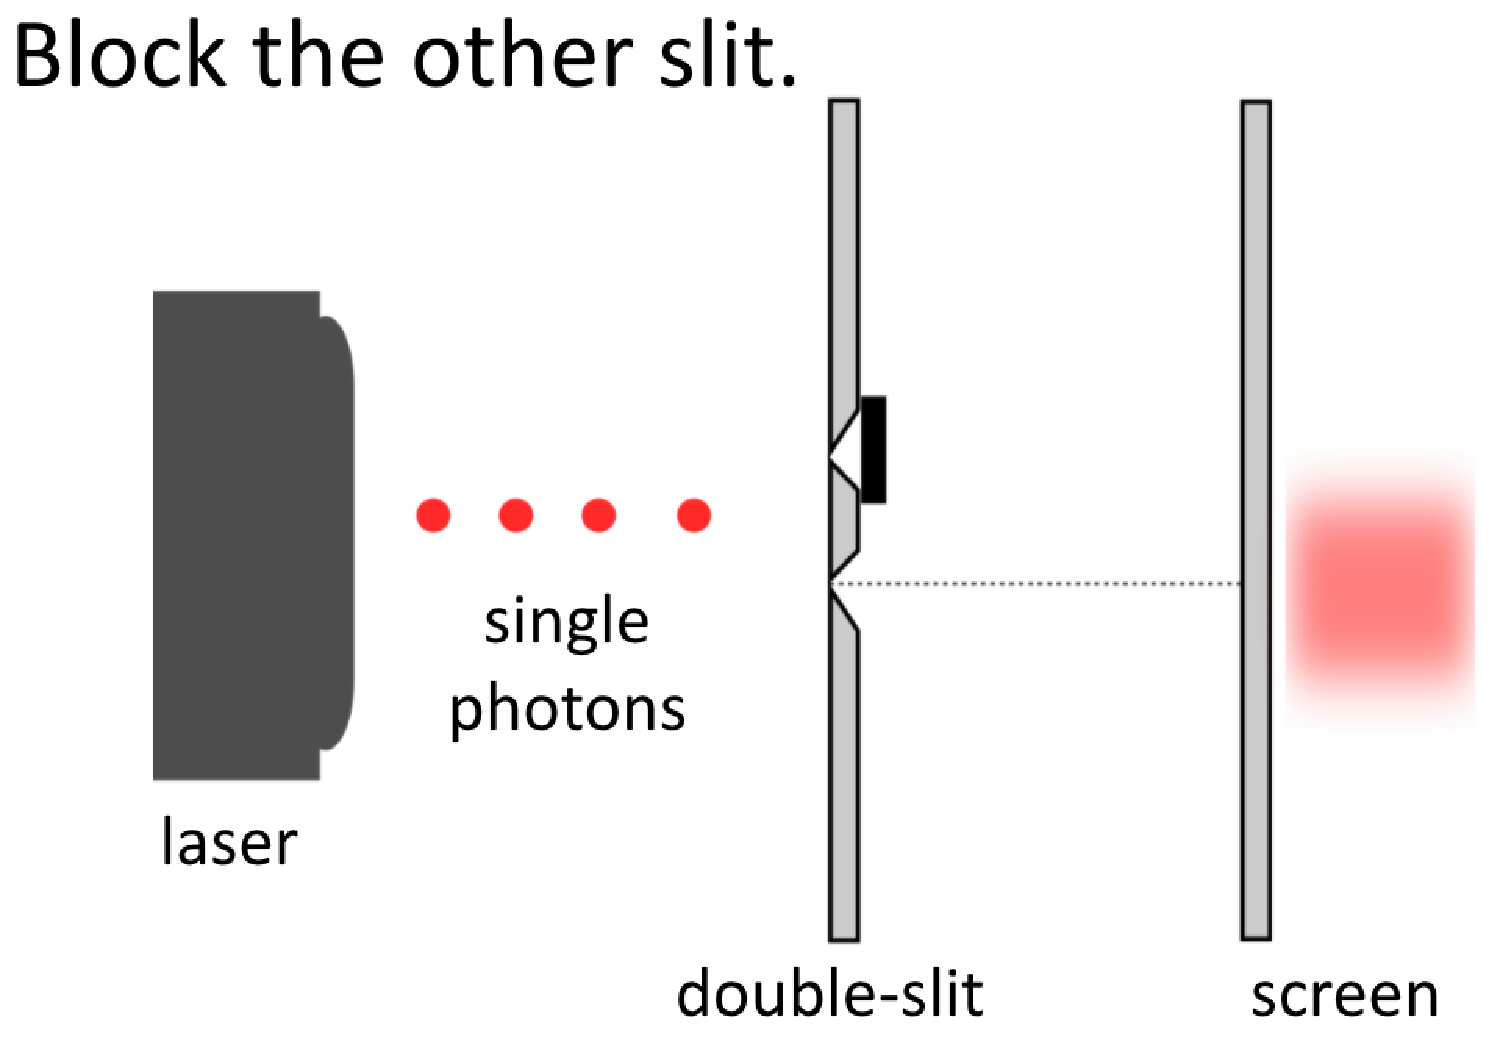
\includegraphics[width=0.8\textwidth]{lesson6/block_top.pdf}
    \label{fig: 1}
    \begin{center}
        \caption{Hole in the top of the block?}
    \end{center}
\end{figure}

% block netiher expectation
\begin{figure}[H]
   \centering
    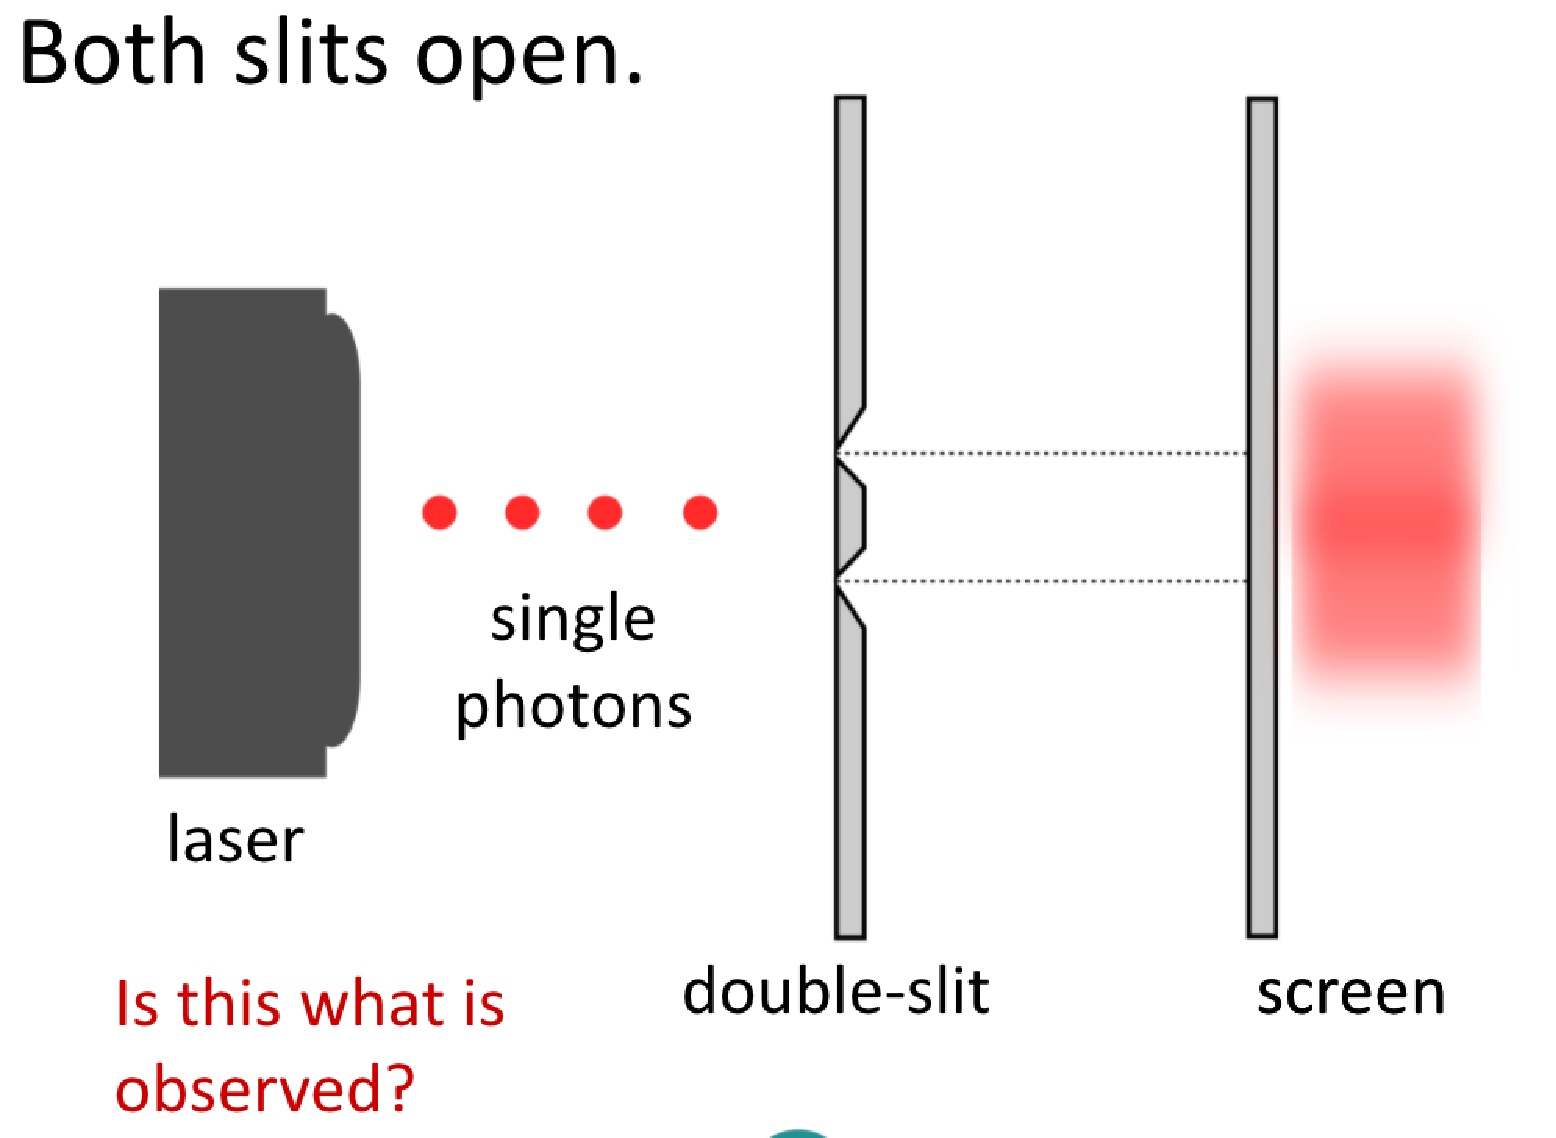
\includegraphics[width=0.8\textwidth]{lesson6/block_neither.pdf}
    \label{fig: 1}
    \begin{center}
        \caption{Neither: the idea?}
    \end{center}
\end{figure}

% block neither reality
\begin{figure}[H]
   \centering
    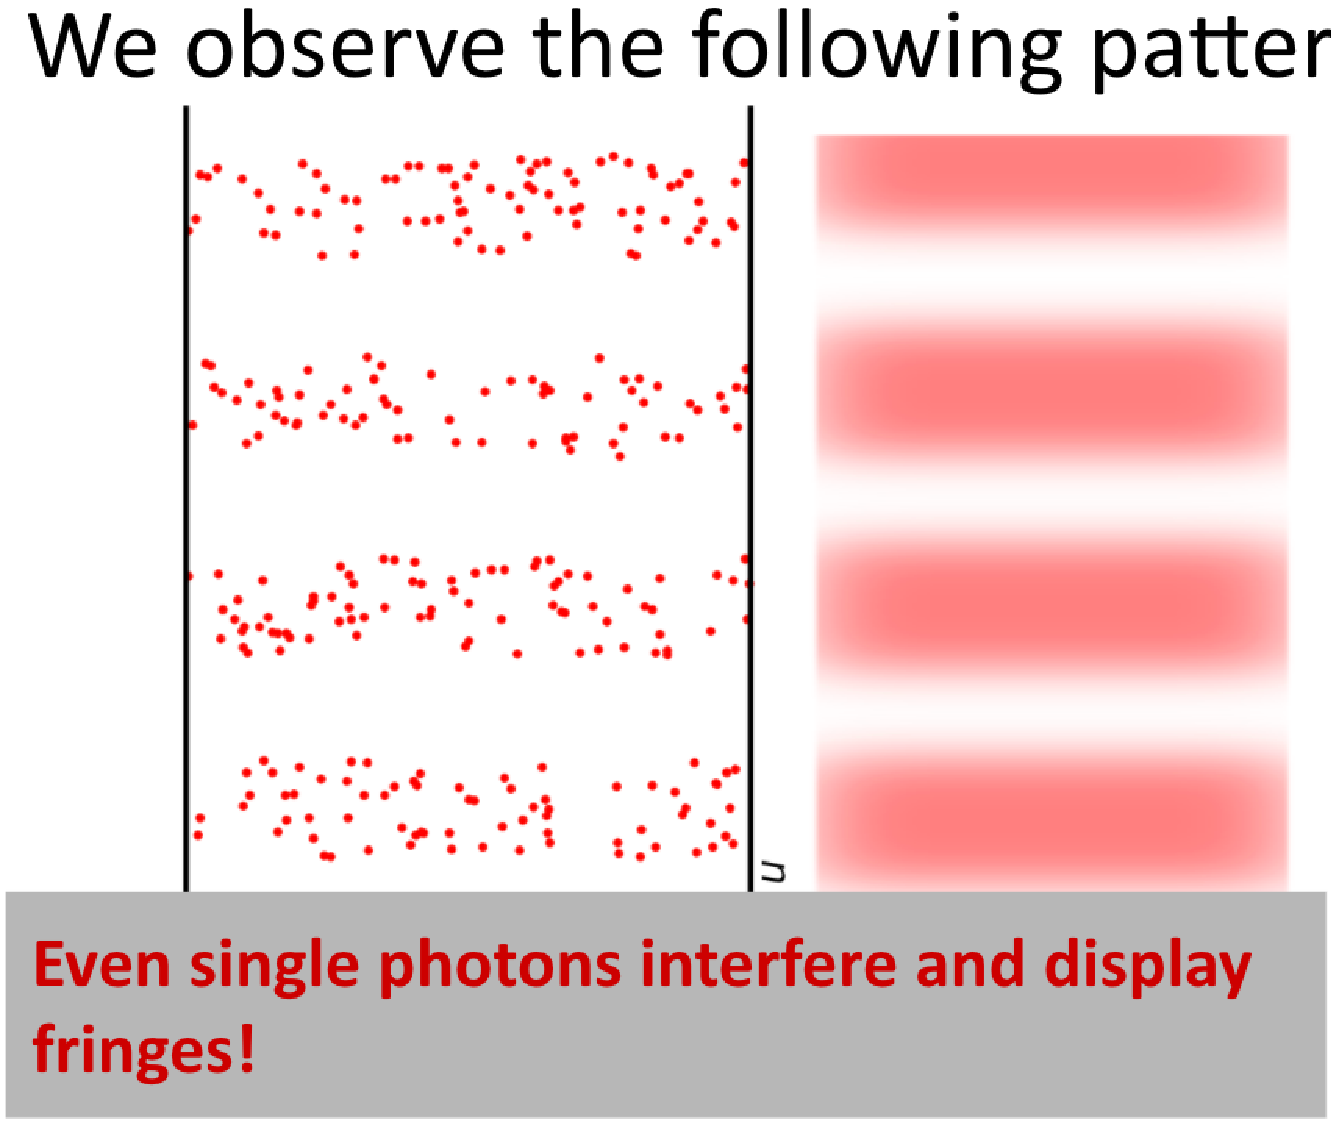
\includegraphics[width=0.8\textwidth]{lesson6/block_neither_reality.pdf}
    \label{fig: 1}
    \begin{center}
        \caption{Neither: the reality?}
    \end{center}
\end{figure}


00:00
step 3 interference with single photons i'm sure you have already seen the the
scenario of a double slit experiment with laser light but let's review it again
in this experiment we've got a source of coherent light so a laser
and it's turned on and the laser light is incident
on a screen where there are only two small double slits where the light
can go through and then it propagates towards another
screen where we detect a pattern and the pattern that we see looks
something like this we've got fringes of bright light and then these white
fringes where there is no light why is that as you can see as the light is
propagating through here these lines they represent the peaks
of the electromagnetic wave whereas the space in between them represent the

00:01
valleys the troughs so as the two waves go through
these slits they have a chance to interfere constructively or destructively
where their peaks meet the wave the interference of the two waves reinforces
their amplitude on the other hand if a peak meets a trough or a valley then the
amplitudes cancel and here we can see these light blue lines
these are the lines along which we see constructive interference
for example here we see the light coming from the top slit
light coming from the bottom slit and they go towards the screen
the path length of these two paths are equal therefore
there is no phase difference between the two two waves coming from

00:02
the top slit and the bottom slit and we observe constructive interference
on the other hand for this other fringe the path length for the for this top
path is a little bit shorter than the bottom one but the phase
difference introduced for this case is exactly 2 pi which
again corresponds to constructive interference as we have seen in the
previous step and similarly for the other fringes for this top one
we have a phase difference of 4 pi on the other hand if we consider these
other parts as we said this is where peaks meet the troughs
so this is where the path differences are odd
integer multiple of pi so for this first dark region on the screen we've got the
path um the phase difference being pi for the second
dark region on the screen we've got the phase difference being 3 pi

00:03
now let's consider the scenario where we attenuate the laser light
to such low levels that it's only firing single photons at a time
and furthermore the level of attenuation is so high
that we can be pretty sure that there's only one photon
at a time between the this screen where we place the double slits
and the screen where we are recording the pattern
so what happens well we know that the photons must go through one of these slits
so let's try and cover one of them what do we expect
if we cover the bottom one then definitely the photons have to go
through the top slit in order to hit the screen so we expect
most of the photons hitting the screen in this region that's the closest to the
top slit on the other hand if we block the top slit
and the photons are allowed to pass through this bottom slit
then we expect most of the photons to be recorded on the screen

00:04
over here what happens if we open both of the slits well they can go through
the top and they can go through the bottom so we
expect something like this we expect that the two previous distributions
are just added together is this really what we see well let's find out
in fact what we see is the following we start firing photos and the screen
originally there's not much pattern that we can discern but
as the time progresses as more and more photons hit the screen we can clearly
see these fringes being formed these fringes
are the same fringes as we could see before with um strong laser light
as shown here so let's just pause and appreciate really what's going on
we saw these fringes on the right with a strong laser light and it wasn't very
surprising however here somehow each individual

00:05
photon knows that they still need to follow the same pattern still they are
drawn towards these bright fringes on the screen
and they avoid these dark fringes in between
them this is because of interference of different possible paths
even though we always have a single photon
in our interferometer still it obeys the same
rules of interference as if we had a strong laser pulse

\section{Interference with qubits}

\begin{equation}
\begin{aligned}
|0\rangle &=\left(\begin{array}{l}
1 \\
0
\end{array}\right) \quad|1\rangle=\left(\begin{array}{l}
0 \\
1
\end{array}\right) \quad H=\frac{1}{\sqrt{2}}\left(\begin{array}{cc}
1 & 1 \\
1 & -1
\end{array}\right) \\
|0\rangle & \longrightarrow H|0\rangle=\frac{1}{\sqrt{2}}(|0\rangle+|1\rangle) \\
& \longrightarrow H\left[\frac{1}{\sqrt{2}}(|0\rangle+|1\rangle)\right] \\
&=\frac{1}{2}(|0\rangle+|1\rangle+|0\rangle-|1\rangle) \\
&=|0\rangle
\end{aligned}
\end{equation}

\begin{equation}
B S 1=\frac{1}{\sqrt{2}}\left(\begin{array}{cc}
1 & 1 \\
1 & -1
\end{array}\right) \quad B S 2=\frac{1}{\sqrt{2}}\left(\begin{array}{cc}
-1 & 1 \\
1 & 1
\end{array}\right) \quad B S 2 \cdot B S 1 \neq I
\end{equation}

\begin{equation}
\begin{aligned}
B S 2 \cdot B S 1|1\rangle &=B S 2 \cdot \frac{1}{\sqrt{2}}\left(\begin{array}{cc}
1 & 1 \\
1 & -1
\end{array}\right)\left(\begin{array}{l}
0 \\
1
\end{array}\right) \\
&=B S 2 \cdot \frac{1}{\sqrt{2}}\left(\begin{array}{c}
1 \\
-1
\end{array}\right) \\
&=\frac{1}{2}\left(\begin{array}{cc}
-1 & 1 \\
1 & 1
\end{array}\right)\left(\begin{array}{c}
1 \\
-1
\end{array}\right) \\
&=\frac{1}{2}\left(\begin{array}{c}
-2 \\
0
\end{array}\right)=-|0\rangle=|0\rangle
\end{aligned}
\end{equation}

% Mach-Zehnder set-up
\begin{figure}[H]
   \centering
    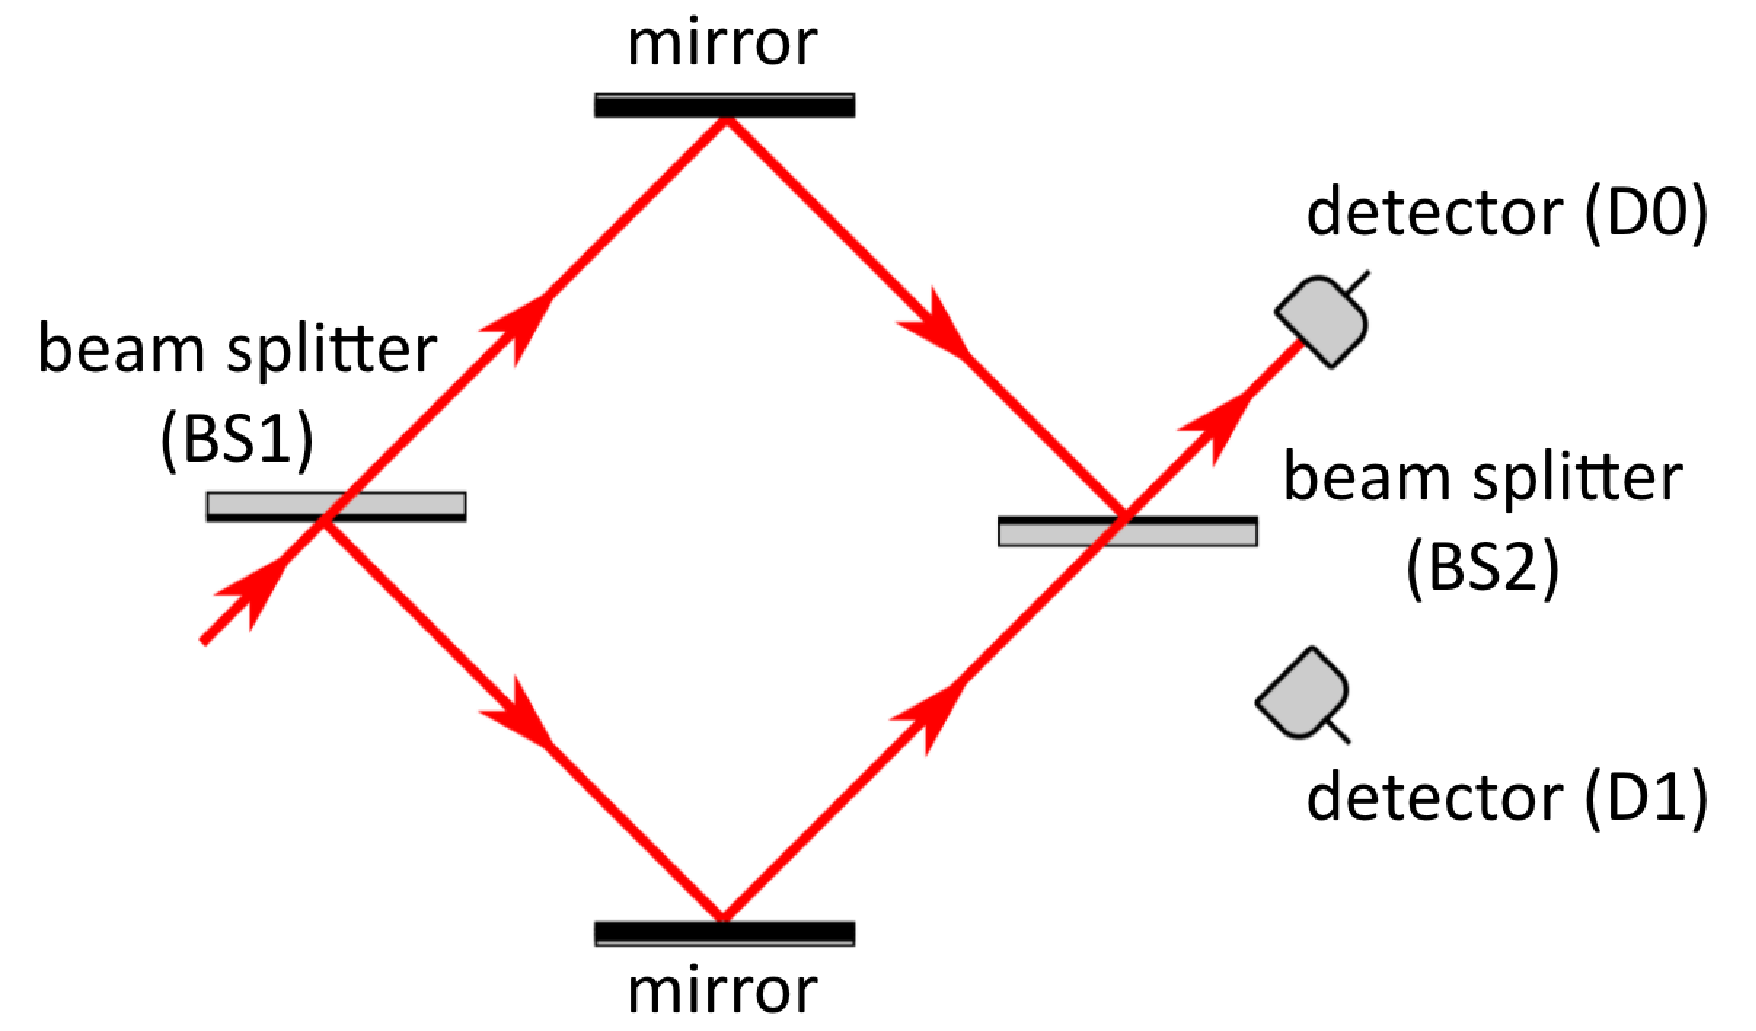
\includegraphics[width=0.8\textwidth]{lesson6/mach_zehnder.pdf}
    \label{fig: 1}
    \begin{center}
        \caption{Mach-Zehnder interferometer.}
    \end{center}
\end{figure}

% Single photon Mach-Zehnder case
\begin{figure}[H]
   \centering
    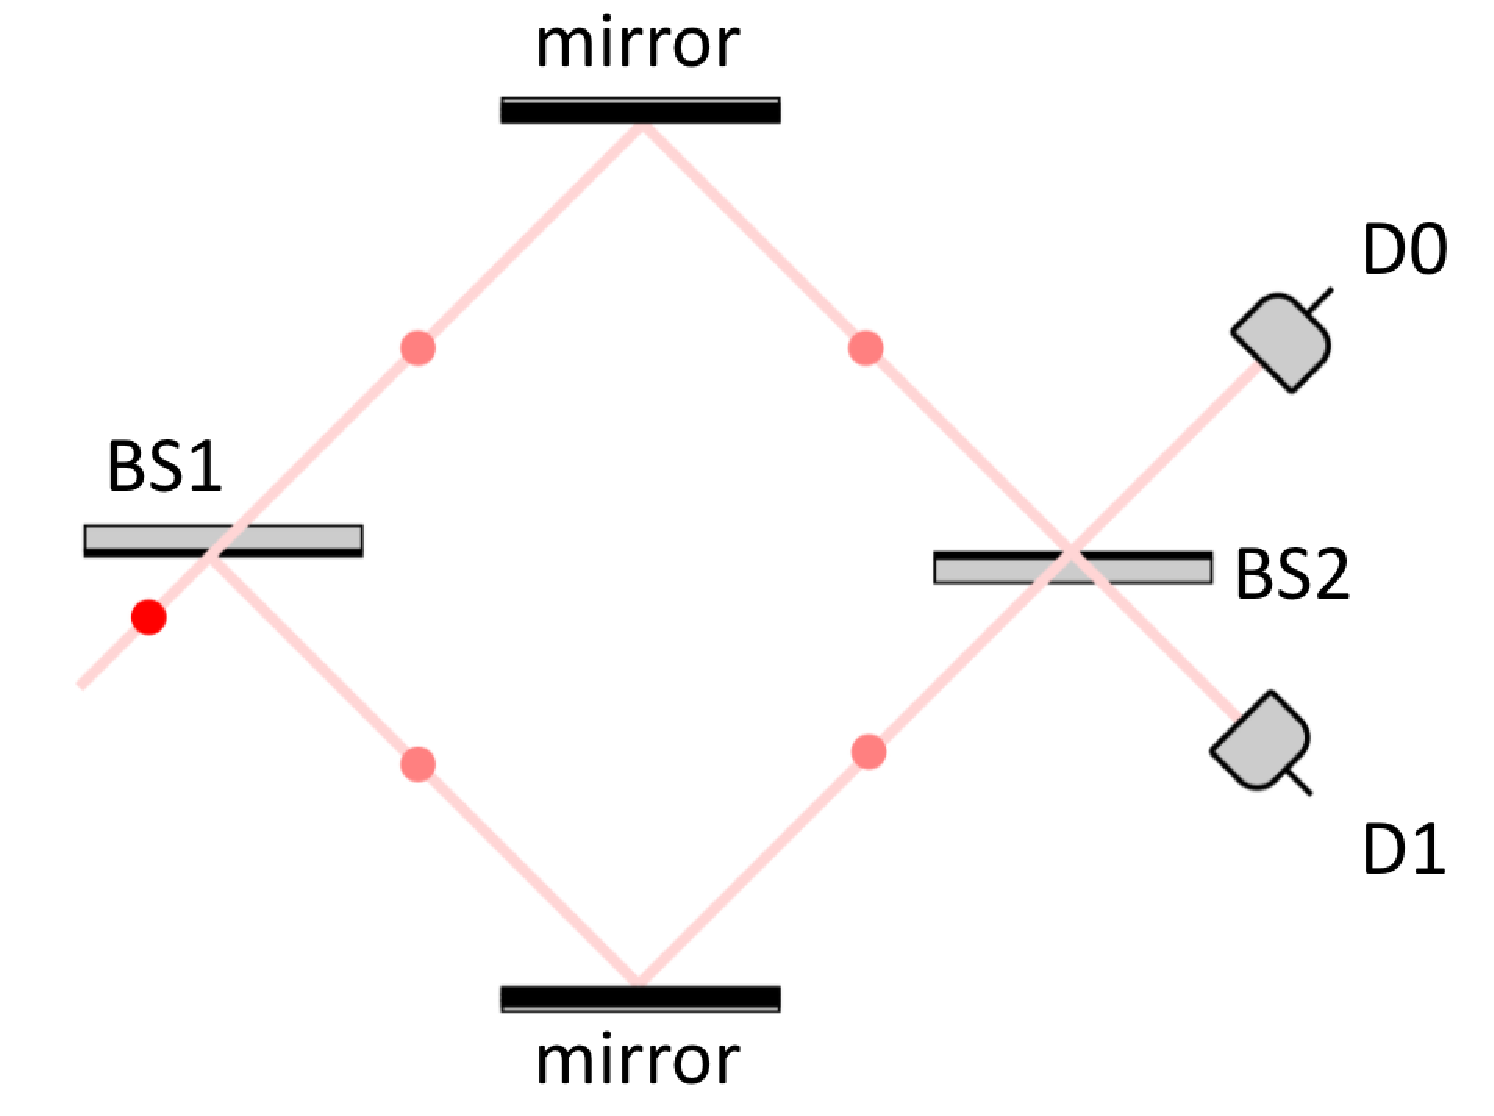
\includegraphics[width=0.8\textwidth]{lesson6/mach_zehnder_single_photon.pdf}
    \label{fig: 1}
    \begin{center}
        \caption{Mach-Zehnder interferometer with a single photon.}
    \end{center}
\end{figure}

% 0 ket top
\begin{figure}[H]
   \centering
    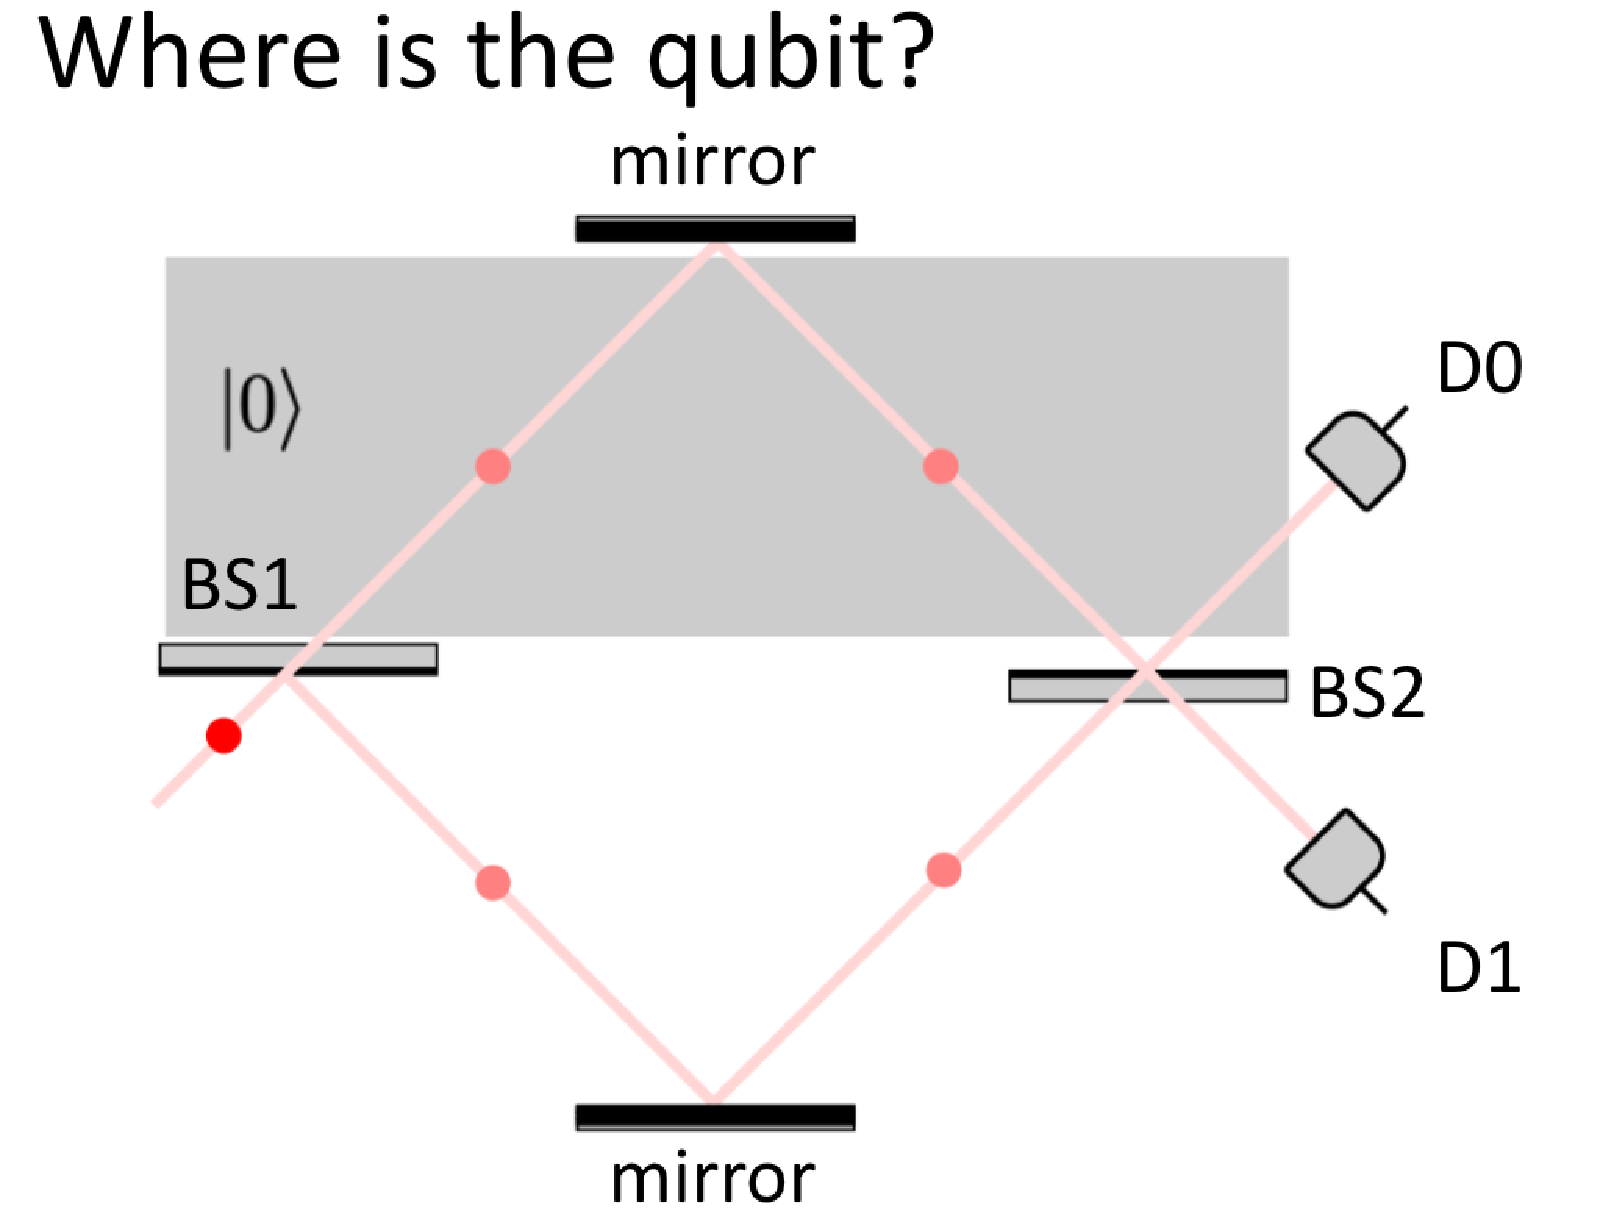
\includegraphics[width=0.8\textwidth]{lesson6/0_ket_botttom.pdf}
    \label{fig: 1}
    \begin{center}
        \caption{$\ket{0}$ state is represented by a photon in the upper path.}
    \end{center}
\end{figure}

% 1 ket bottom
\begin{figure}[H]
   \centering
    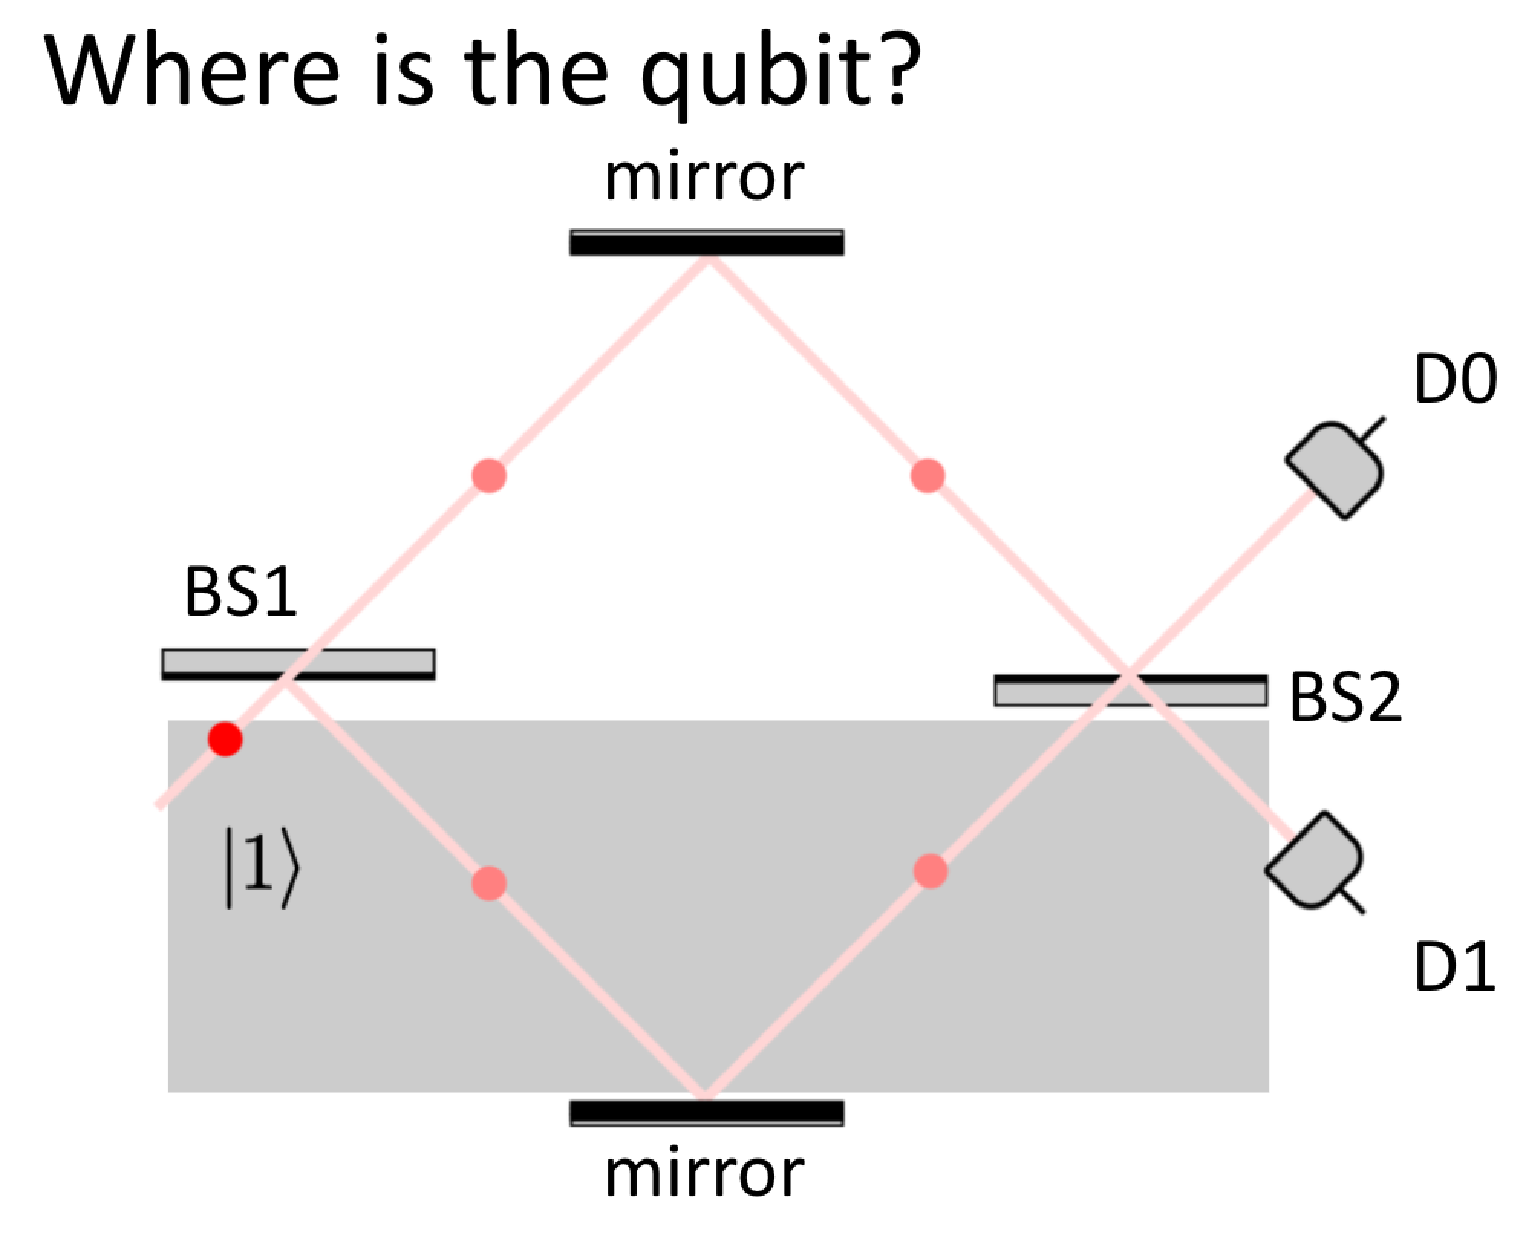
\includegraphics[width=0.8\textwidth]{lesson6/1_ket_bottom.pdf}
    \label{fig: 1}
    \begin{center}
        \caption{$\ket{1}$ state is represented by a photon in the lower path.}
    \end{center}
\end{figure}

\begin{equation}
B S 2 \cdot B S 1|1\rangle=|0\rangle
\end{equation}

% D0 always clicks
\begin{figure}[H]
   \centering
    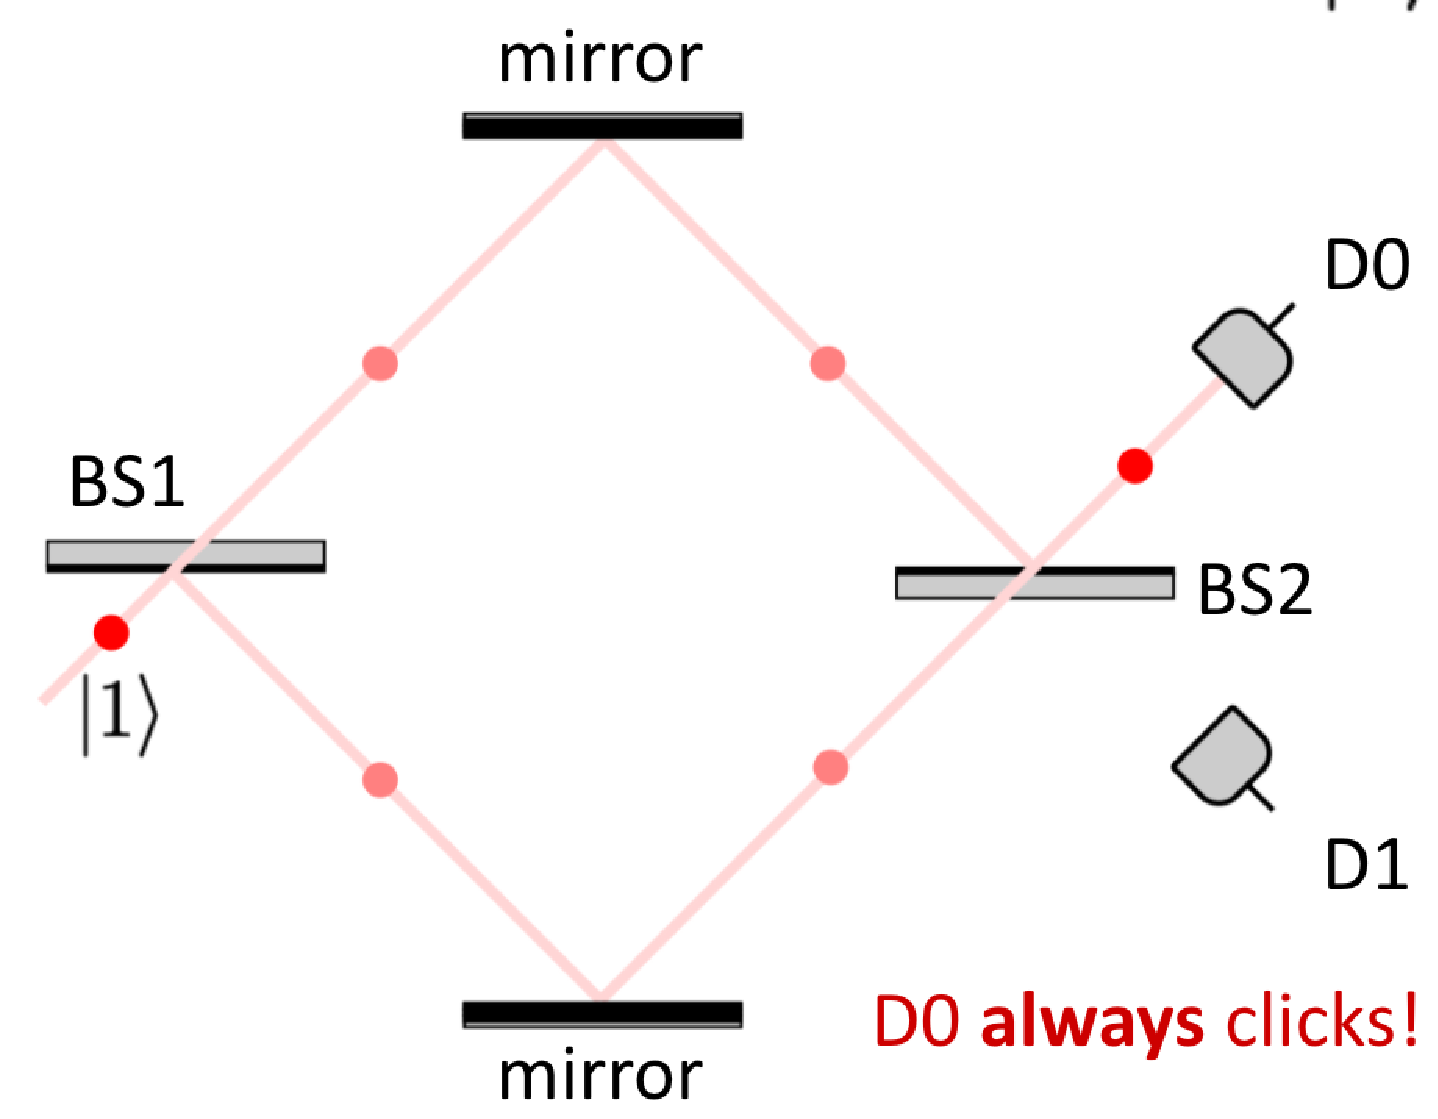
\includegraphics[width=0.8\textwidth]{lesson6/d0_always_clicks.pdf}
    \label{fig: 1}
    \begin{center}
        \caption{$D0$100\% probability.}
    \end{center}
\end{figure}

% block bottom path
\begin{figure}[H]
   \centering
    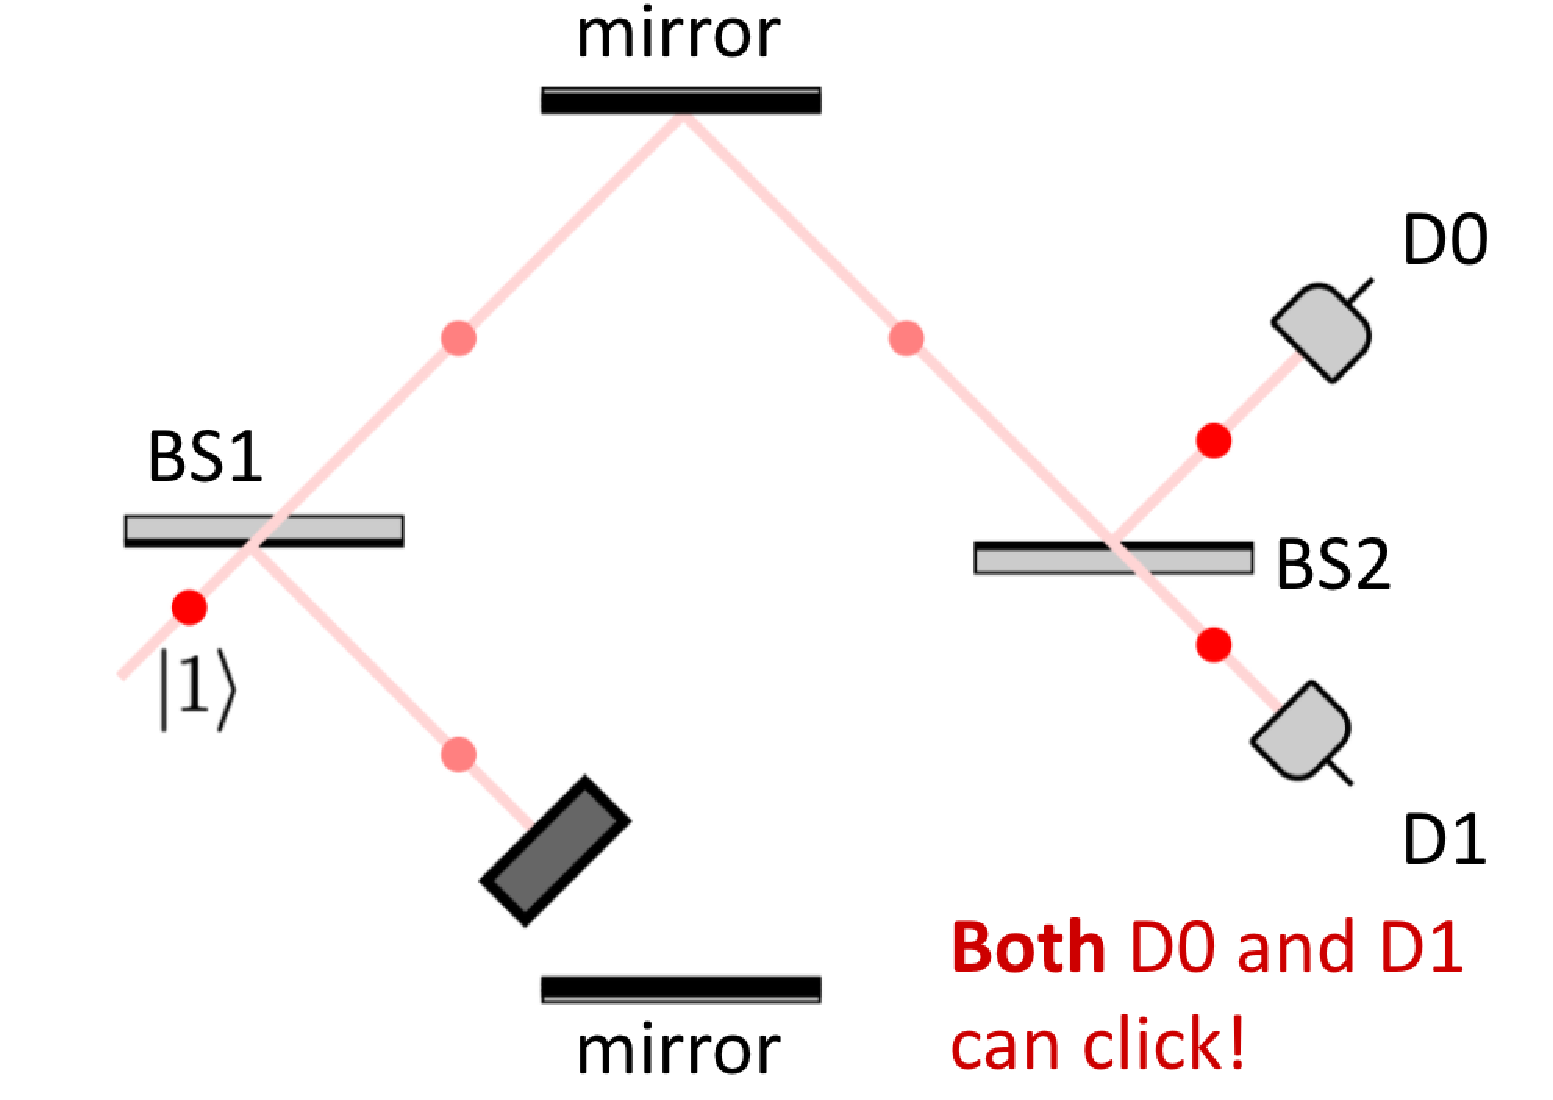
\includegraphics[width=0.8\textwidth]{lesson6/bottom_blocked.pdf}
    \label{fig: 1}
    \begin{center}
        \caption{Lower path blocked.}
    \end{center}
\end{figure}


00:00
step 4 interference with qubits so we have seen how light interferes how
waves interfere and even how single photons interfere we can in fact see
interference also with single qubits let's see how
consider that we have a hadamard gate and we apply it on the state of a qubit
so we will consider two states one is our state 0 which is given by this state
vector another one is one which is given by its orthogonal
friend zero one and the hadamard gate is given by this transformation matrix
if we start in the state zero and apply the hadamard gate to it
what we get we have seen that already is we get it and we create an equal
superposition of state 0 and 1. now we can do the same thing again we
can apply another hadamard gate to this superposition and see what

00:01
actually happens applying the hadamard to the state 0
creates another superposition of 0 and 1
over here 0 plus 1 and applying hadamard gate to the state one
creates a superposition of zero and one but this time
with the one having a minus minus probability amplitude in front of it so after
applications of two hadamard gates this is our state you can see
that these terms they both have a positive probability amplitude
plus a half plus a half whereas the other two terms have opposite
amplitudes they've got plus a half and negative a half so the effect of that
is that the probability amplitudes for one's cancel
whereas the probability amplitudes for the zeros they
constructively interfere and we end up in a state 0 which was our initial state

00:02
and this works also for state 1 if we use that as an initial state but this time
the cancellation of probability amplitudes happens for the zero terms
because they have they have plus one half minus one half
and the one terms they constructly interfere because both of them have
plus a half plus a half probability amplitudes
so this may not surprise you too much after all
applying hadamard twice actually applies the identity
which is doing nothing that's because the hadamard gate is its own inverse
so let's consider different transformations that do not have this property in
particular let's go consider two transformations let's call them bs1
and bs2 you can see that bs1 is actually our previous hadamard gate but let's
just keep calling it bs1 for reasons that will become
apparent a little bit later and this bs2 looks a little bit similar like a

00:03
hadamard gate but this time the minus is not located over here but
it's over there but you can check for yourselves that
applying these gates in sequence is not the same thing as doing nothing
in particular bs2 times bs1 is not equal to the identity
but let's see what happens again we take our initial state
let's say our initial state is 1. we first apply the transformation bs1 and
what we get is the following we apply the hadamard gate to the vector 0 1
and after simple multiplication we got the following state
vector which is just a superposition of 0 minus
and then we continue applying our gates this time we apply bs2 and what we get

00:04
is in fact another translation you see over here the probability amplitudes
corresponding to state zero they constructly interfere
whereas the probability amplitudes uh contributing towards state one
they destructively interfere and therefore the probability amplitude for state 1
becomes 0. this minus term that appears here is not important and has no
consequence because it's just a global face so we can just ignore it
now let's consider an optical instrument called a max sender interferometer
it consists of two beam splitters which are bs1
and bs2 and two mirrors over here and over here and two detectors
and the games that we like to play with this mark zender interferometer is that
we we feed in some light into the first beam splitter
and then we ask the questions when will d0 click when will detector d1 click
what's the intensity measured detector d0 was the

00:05
intensity measured at detected d1 and so on in this particular case
we assume that we only have light coming in from the bottom over here and the
mirrors and beam splitters are set in such a way that the path lengths
are the same here what can happen is the light can be
reflected from the first beam splitter bounce of the mirror and enter the
second beam splitter or it can be transmitted through the first beam splitter
bounce of the top mirror hit the second beam splitter
interfere with the beam coming from the bottom branch
and either it will be detected at d0 and d1
if the path lengths are the same then for this scenario it will always be
detected in d in this top detector d0 now let's consider that we have again

00:06
only a single photon entering our max ender interferometer
and then again the single photon can be reflected at the first one or
transmitted it bounces off the mirrors which don't
really do anything they just alter the path of the photon
and then it recombines at the second beam splitter and we ask the question
does it get detected at d0 or does it get detected at d1
also the max and the interferometer implements our qubit how where is the qubit
well if the photon is found in the top half
of the interferometer we say that it's in the state zero
on the other hand if it's found in the bottom half we say that it's in the
state one so here the different paths encode different
computational states of the qubit so let's consider our initial state to

00:07
be in state 1 meaning it enters our max center
interferometer from the bottom half and in fact now you see why we have
called those previous transformations bs1 and bs2 they
correspond to the mathematical description of how these beam splitters uh
affect the probability amplitudes of our qubit and we proved before that
if we first act on our qubit on our initial state
with beamsplitter1 and subsequently with beamsplitter 2
then we know that if the initial state is in the bottom half
then the output state will always be found in the top half
meaning d0detector always clicks but yet again the situation is very
similar to the previous step here there is only a single photon found
in the maxender interferometer and we cannot divide
photons there's always just one yet somehow it knows that it has to

00:08
interfere with itself and always goes towards a detector d0
now let's do a simple test let's actually put some absorbing material
and block the possibility of the photon going through the lower half of the max
and the interferometer what do we see well the photon can
coming in here can get reflected if it does get reflected
then it just gets absorbed and we don't get any clicks
however if it gets transmitted then it goes through it bounces off the mirror
and it uh it is incident onto the second beam splitter
where again it has an equal probability of being reflected or passing through
the beam splitter therefore it has a probability of being detected by both
detected detector d0 and the detector d1 so what we have effectively done by

00:09
blocking this path of photon in the bottom of the max and the interferometer
interferometer is we have prevented interference from taking place
at beam splitter two that is why we see both possibilities d0 and d1


\newpage
\begin{exercises}
\exer{Consider the following quantum state:}
\begin{equation*}
\ket{\psi} = \frac{\sqrt{3}}{2}\ket{0} + \frac{1}{2}\ket{1}
\end{equation*}
\subexer{Find the probability of measuring a zero.}
\subexer{Find the probability of measuring a one.}


\end{exercises}

